% ==================================================================
%               FORMATO DE TESIS DE LICENCIATURA UAIE
% ==================================================================
% Este formato de tesis fue diseñado por Manuel Reta Hernández como
% modelo de documento de tesis de licenciatura, propuesto para la
% Unidad Académica de Ingeniería Eléctrica de la Universidad Autónoma
% de Zacatecas.
% El archivo utiliza el paquete uaztesism.cls y fue adaptado de los
% paquetes de tesis de "the Purdue University" y de "the University of
% Wisconsin-Madison".

% ==================================================================
% INICIA PREÁMBULO DEL DOCUMENTO
% ==================================================================

% -----------DECLARACIÓN DE TIPO DE DOCUMENTO A DISEÑAR-------------

\documentclass[12pt,tesis]{uaztesis}

% --------------DECLARACIÓN DE PAQUETES A UTILIZAR------------------
%(se pueden agregar a la lista cuantos paquetes sean necesarios)
\usepackage[latin1]{inputenc}
\usepackage[nottoc]{tocbibind}
\usepackage{amssymb,amsmath,amsfonts}
\usepackage{color,graphicx,curves}
\usepackage{subfigure}
\usepackage{multirow,rotating}
\usepackage[T1]{fontenc}
\usepackage{hyperref}
\usepackage{float}


% --DECLARACIÓN DE RUTA DE CARPETA DONDE SE ENCUENTRAN LAS FIGURAS--
\graphicspath{{Figuras/}}

% --------------OPCIONES DE IMPRESIÓN DE FIGURAS--------------------
% Con la instrucción \psdraft se crea un espacio en blanco en donde van
% las figuras. Esto ahorra toner en la impresión del borrador de tesis.
%
% Con la instrucción \psfull se incluyen a todas las figuras.
\psfull

% --------------DECLARACIÓN DEL ESTILO DE PÁGINA--------------------
% El estilo de página \pagestyle{thesis} coloca los encabezados
% correctos de la versión final del documento.

\pagestyle{thesis}
%\noappendixfigures
\noappendixtables


% ===================================================================
% INICIA EL CONTENIDO DEL DOCUMENTO
% ===================================================================

\begin{document}

% Para opción de tesis de licenciatura
\thesis

% Introducción en sílabas de palabras desconocidas por LaTeX
% Declaración de número de páginas en números Romanos
\clearpage\pagenumbering{roman}

% ------------------INTRODUCCIÓN DE DATOS----------------------------

% Título de la tesis, autor, y grado a recibir:
\title{Estimaci\'on de par\'ametros morfol\'ogicos en rocas sedimentarias usando Fourier el�ptico y redes neuronales}
\author{Erik Mej\'ia Hern\'andez}
\degree{Maestr\'ia en Ciencias del Procesamiento de la Informaci\'on}
\carrera{Ingenier\'ia El\'ectrica}

% Grado y nombre de asesores de tesis:
\advisortitle{Dr.} \advisorname{Jos\'e de Jes\'us Villa Hern\'andez}
\gradoasesor2{Dr.} \nombreasesor2{Gamaliel Ch\'avez Moreno}

% Fecha de solicitud de tema de tesis:
\fechasol{12 de septiembre de 2008}

% Fecha de aprobación de tema de tesis:
\fecharev{18 de octubre de 2008}

%Fecha de autorización de impresión de tesis:
\fechaaut{19 de enero de 2009}

% Fecha de Examen profesional:
\date{Algun dia de 2020}

% Grado y nombre de director de la Unidad Académica:
\dirtitle{M. en C.} \dirname{José Manuel Cervantes Viramontes}

% Grado y nombre de los tres vocales restantes, miembros del jurado:
\vocalbtitle{Dr.} \vocalbname{Jorge de la Torre y Ramos}
\vocalctitle{Ing.} \vocalcname{Amando Castañeda Carrillo}
\vocaldtitle{M. en A.} \vocaldname{Manuel Haro Macías}

% ---------GENERACIÓN DE PÁGINAS PRELIMINARES DEL DOCUMENTO----------

% Genera página de presentación
\maketitle

% Genera oficio de autorización de tema de tesis
%\begin{revision}
%\end{revision}

% Genera oficio de autorización de impresión de tesis
%\begin{autorizacion}
%\end{autorizacion}

% Genera oficio de aprobación del Examen
%\begin{aprobacion}
%\end{aprobacion}

% Genera páginas de resumen
%\begin{resumenespa}
%  \input{resumen}              % incluye al archivo resumen.tex
%\end{resumenespa}

% Genera página de dedicatoria (opcional)
%\begin{dedicatoria}
%  \input{dedicatoria}          % incluye al archivo dedicatoria.tex
%\end{dedicatoria}

% Genera página de agradecimientos (opcional)
%\include{agradecimientos}      % incluye al archivo agradecimientos.tex

% Genera páginas del contenido general y lista de figuras y tablas
\tableofcontents
\renewcommand{\listfigurename}{Lista de Figuras}
\listoffigures                 % se indica sólo si hay figuras

%\listoftables                  % se indica sólo si hay tablas

% Genera páginas del nomenclatura
%\include{nomenclatura}    % incluye al archivo nomenclatura.tex

%--------INCLUSIÓN DE LOS ARCHIVOS (CAPÍTULOS) DEL DOCUMENTO--------

% Declaración de número de páginas en números Arábigos
\clearpage\pagenumbering{arabic}

\chapter{Introducci�n}

%\lipsum[1]
%\begin{figure}[!htb]
%	\captionsetup{singlelinecheck = false, format= hang, justification=raggedright, font=footnotesize, labelsep=space}
%	\centering
%	\begin{measuredfigure} % \begin{measuredfigure}
%		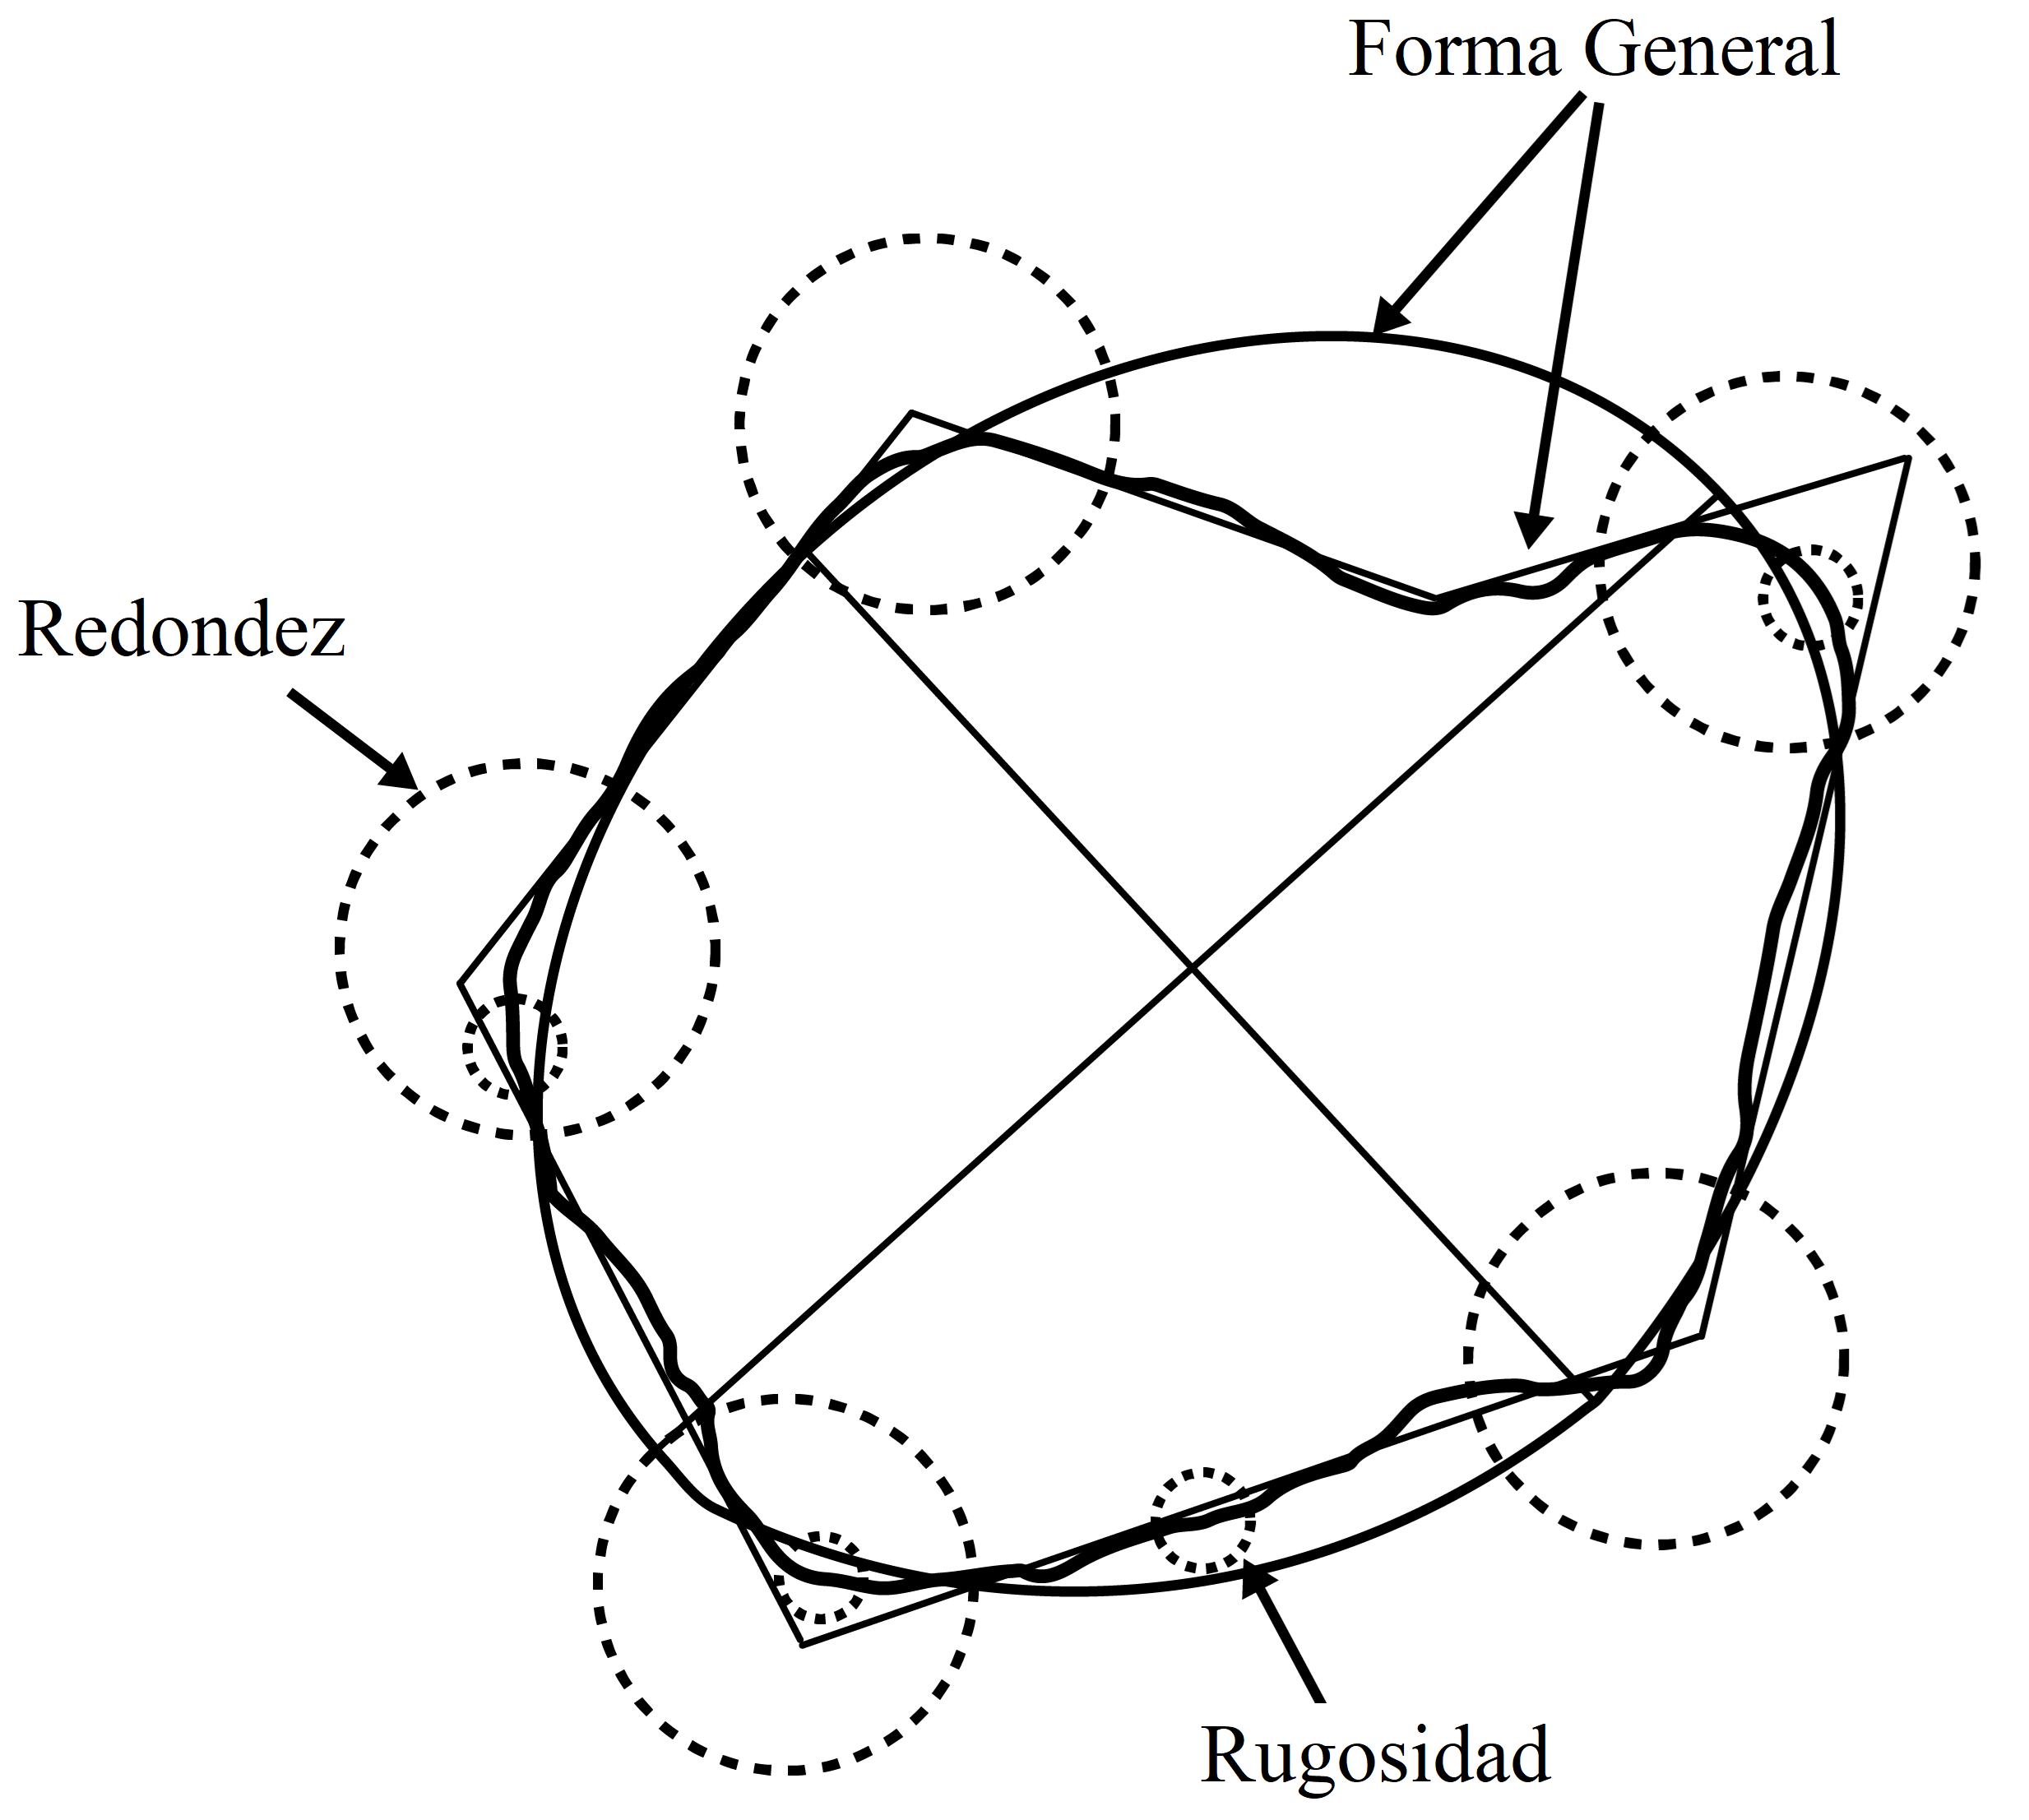
\includegraphics[scale=.2]{figuras/fig1.png}
%		\caption{Chuck Jones ? Pepe Le Pew in action}
%	\end{measuredfigure}
%	\label{PlP}
%\end{figure}
%\lipsum[2]

\section{Antecedentes}  

Nuestro planeta puede ser visto como un sistema conformado por la hidrosfera, atm�sfera, biosfera y tierra s�lida. El componente principal de la tierra s�lida son las rocas \cite{Lutgens2005}.  Las rocas son agregados naturales de uno o m�s minerales. Estas pueden clasificarse por su origen y proceso en tres clases: �gneas, metam�rficas y sedimentarias \cite{schon2015physical}. Las rocas �gneas son las que se forman a partir del enfriamiento de minerales fundidos (magma) entre la corteza terrestre y el manto superior. Las rocas �gneas algunas veces pueden alcanzar la parte superior de la  corteza terrestre por medio de volcanes o por el ascenso de capas de la corteza. En la corteza existe un proceso llamado meteorizaci�n que consiste en la fragmentaci�n de rocas por alteraciones f�sicas y qu�micas (como la gravedad, erosi�n, materia org�nica). Estas rocas se transportan generalmente por gravedad y se depositan en las zonas m�s bajas de la corteza terrestres (la mayor�a en los oc�anos). Estos sedimentos son nuevas rocas y se les conocen como rocas sedimentarias. Las rocas metam�rficas se generan a partir de rocas �gneas, sedimentarias o mismas rocas metam�rficas. Como su nombre lo indica estas rocas se generan por el cambio (metamorfosis) de una roca madre, este cambio es generado por altas presiones y temperaturas, pero sin que lleguen a fundirse \cite{Lutgens2005}. 

De estos tres tipos de rocas, las m�s importantes son las rocas sedimentarias por las siguientes razones: (1) representan el 80\% de la corteza terrestre, (2) permiten conocer los procesos e historia de la tierra, (3) son de gran importancia en el sector econ�mico porque de ellas derivan el petr�leo, gas natural, carb�n, sal, azufre, potasio, yeso, caliza, fosfato, uranio y m�s minerales \cite{Boggs2013}, (4) en algunos casos representan un riesgo para poblaciones como la asentadas en las cercan�as de volcanes o grandes sedimentos, (5) en el estudio de suelo para la construcci�n \cite{Rodriguez2013}.  

Las rocas sedimentarias se estudian por su composici�n f�sica, qu�mica  y mineral�gica. El estudio f�sico se conforma por tres par�metros; tama�o, morfolog�a y orientaci�n. El conocer estos par�metros nos permite deducir su origen, los diversos procesos transporte, el entorno reol�gico y clim�tico y su deposici�n. Para medici�n de tama�o y la orientaci�n existen diversas t�cnicas muy bien establecidas y muy precisas \cite{tucker2009sedimentary}. Por otro lado la morfolog�a es un concepto reciente, en comparaci�n a los otros y a�n se encuentra en desarrollo y b�squeda de conceptos universales \cite{DIEPENBROEK1992}.  

La morfolog�a describe la forma (shape) de objetos o part�culas mediante mediciones de su contorno. La morfolog�a no s�lo es importante en el estudio de rocas sedimentarios sino que se extienda a otros campos cient�ficos y productivos como la nanomedicina, agricultura, biolog�a, neurociencias, arte visual, entre otros (\cite{da2009shape}, \cite{Shah2011}, \cite{toy2014shaping}). En general, ha sido importante para entender y estudiar el porque tienen cierto aspecto externo todos y cada uno de los objetos o seres vivos. La morfolog�a de rocas sedimentarias se describe por tres par�metros: forma general (form), redondez (roundness) y textura superficial (roughness), los cuales se relacionan con procesos geol�gicos. Estos tres par�metros son jer�rquicos y de escalas diferentes, por lo que uno no afecta al otro. La forma es la caracter�stica de mayor jerarqu�a que est� relacionada con los aspectos m�s generales. La forma se calcula mediante relaciones axiales adimensionales o relaciones de circularidad. La redondez es una caracter�stica intermedia superpuesta a la forma. El grado de redondez o angularidad est� relacionado con las curvas y las esquinas principales del contorno. La rugosidad o textura se refiere a irregularidades m�s finas superpuestas en la redondez y la forma \cite{BARRETT1980,Blott2008,M.C.Powers1953}. Estas propiedades se muestran en la Figura~\ref{fig:fig1}.

\begin{figure}[H]
	
	\centering
	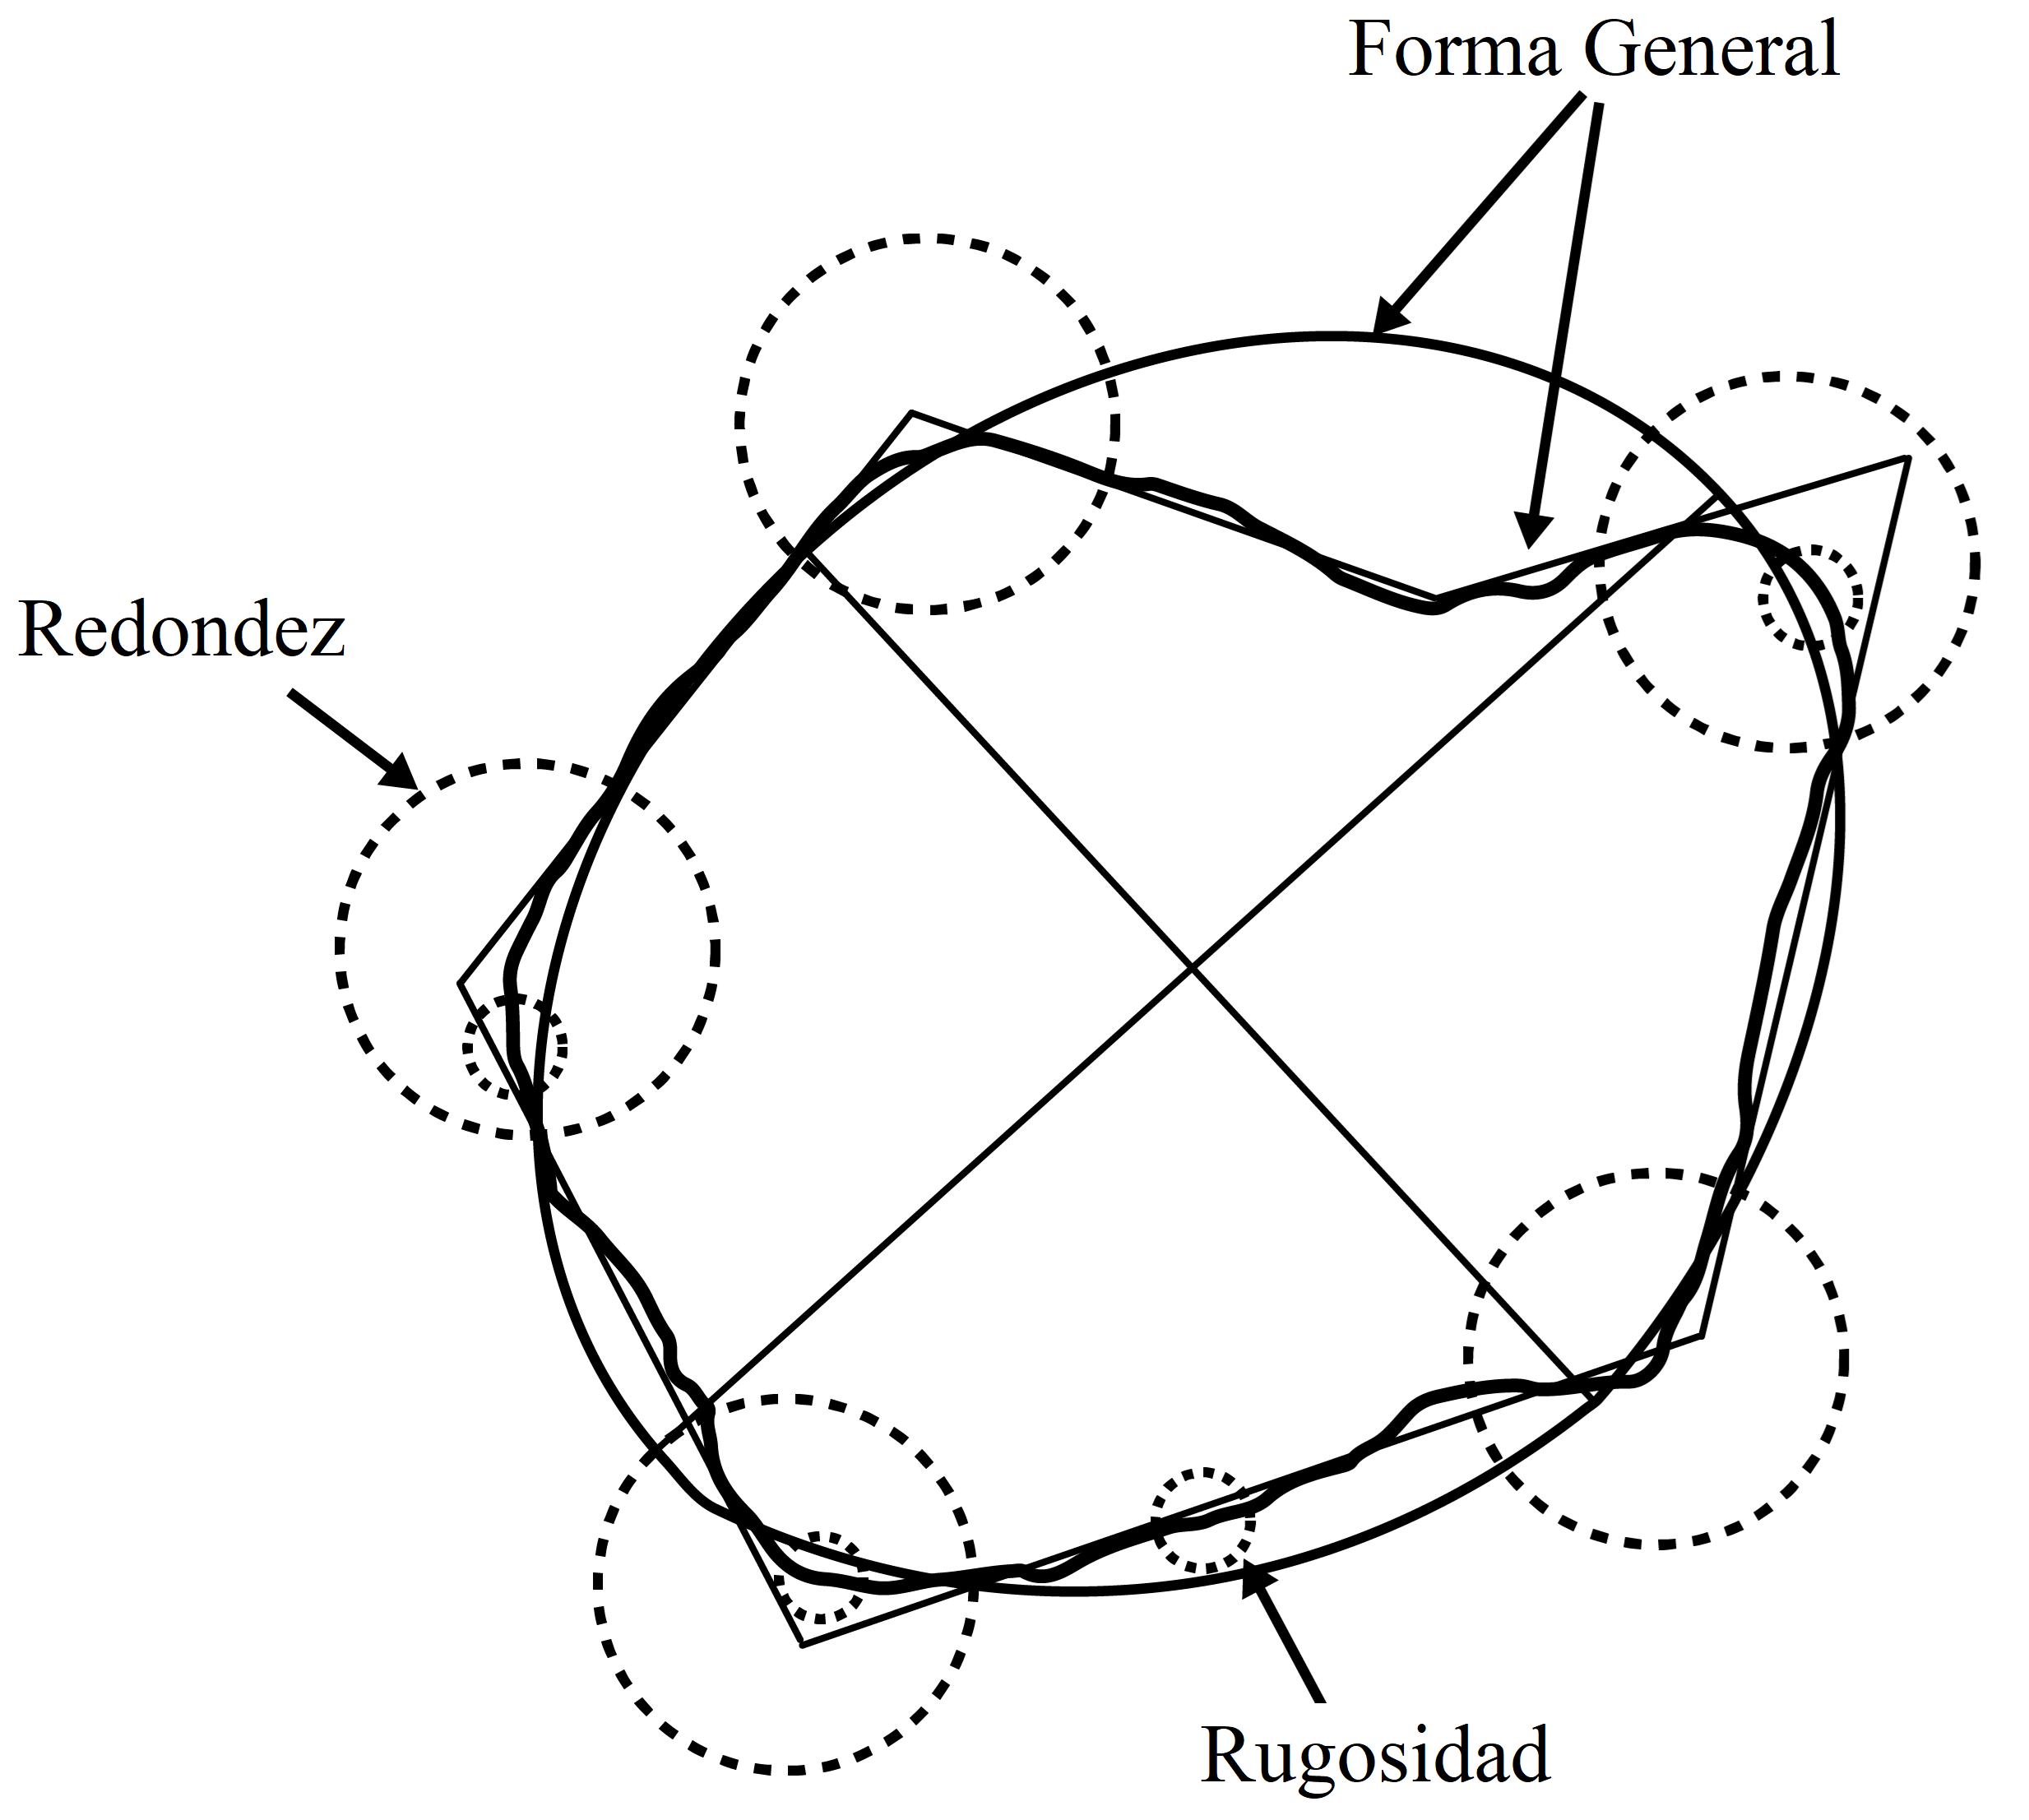
\includegraphics[scale=.2]{figuras/fig1.png}
	\caption{Forma, redondez y textura superficial propuestas por Barrett \cite{BARRETT1980}. }
	\label{fig:fig1}
\end{figure}

Existen diversas expresiones para medir la forma, una de las m�s usadas en el campo geol�gico es la propuesta por Wadell\cite{Wadell1935}, la cual se obtiene de la relaci�n entre el radio del c�rculo cuya �rea es igual a la de la part�cula y el radio del c�rculo m�s peque�o que inscribe a la part�cula \cite{Wadell1935}. Existen tres enfoques para medir la redondez; los basados en curvatura, los que emplean Fourier y los relacionados con Fractales.  El m�todo basado en curvatura es simple y preciso, sin embargo es un m�todo que depende de la escala. Los m�todos basados en Fourier son muy populares sin embargo analizar el espectro es complicado y de un alto costo computacional. El uso de fractales para describir la forma se ha vuelto popular sin embargo tiene problemas para identificar algunos tipos de redondez y son muy sensibles al suavizado de contornos.

En la presente tesis planteamos usar redes neuronales para estimar la forma y redondez de rocas sedimentarias. La variable de entrada a la red neuronal son los coeficientes de las series Fourier El�ptico. Se eligi� este m�todo de transformaci�n por ser invariante a la escala, a la rotaci�n y traslaci�n.  Como objetivo para la forma se emple� la circularidad propuesta por Wadell \cite{Wadell1935}. Para la redondez, se eligi� como objetivo el grado de angulosidad calculado con el m�todo propuesto por Wadell \cite{wadell1933sphericity}, el cual define el grado de redondez como la relaci�n entre el radio de curvatura promedio de las esquinas de una part�cula y el radio del c�rculo circunscrito m�s grande posible. Se probaron diversas arquitecturas de red, y la mejor configuraci�n para calcular la redondez fue: una red neuronal profunda de 6 capas, la capa de entrada con la misma cantidad de neuronas que los datos de entrada y funci�n de activaci�n Sigmoide, 4 capas ocultas con una cantidad de neuronas que se iba reduciendo la mitad de la capa anterior, con funci�n de activaci�n Sigmoide. La capa de salida con una sola neurona con funci�n de activaci�n Sigmoide. La base de datos para entrenar la red neuronal se compone de 1123 im�genes de rocas reales de diversos fen�menos geol�gicos. La red neuronal tiene un error de m�nimos cuadrados de 5e-03 con los datos de entrenamiento. El resultado fue comparado con clasificaciones visual realizadas por Krumbein y Sloss. La red neuronal propuesta es invariante a la escala, rotaci�n y traslaci�n, adem�s de permitirnos tener la redondez y la circularidad 2800 veces m�s r�pido que el m�todo de Wadell \cite{Wadell1935}. 


\section{Planteamiento del problema de investigaci�n}
\label{Sec12}

Los m�todos para medir la forma general y redondez no son invariantes a la escala, rotaci�n y traslaci�n. Los m�todos basados en Fourier son invariantes a estas 3 transformaciones, sin embargo el tratamiento del espectro son es una tarea f�cil. Por lo que no existe un m�todo invariante y f�cil de ajustar.


\section{Justificaci�n del problema de investigaci�n}

El an�lisis morfol�gico de las rocas sedimentarias es importante en geolog�a para la reconstrucci�n hist�rica de nuestro planeta. Tambi�n es importante en sectores econ�micos y de prevenci�n de riesgo. A pesar de ser un an�lisis muy utilizado no existe un m�todo que sea invariante a la escala, rotaci�n y traslaci�n, as� como preciso, f�cil y r�pido de usar. 


\section{Preguntas de Investigaci�n}
\begin{itemize}
	\item �Ser� capaz una red neuronal profunda de modelar el algoritmo de Zheng \cite{Hryciw2016} que usa el m�todo de Wadell \cite{wadell1933sphericity}?
	\item �Cu�les ser�n las arquitecturas de red neuronal profunda capaces de estimar la redondez y circularidad de los contornos de rocas sedimentarias?
\end{itemize}

\section{Hip�tesis}
Una red neuronal profunda es capaz estimar la redondez independientemente de la escala, rotaci�n y traslaci�n con una velocidad mayor que el algoritmo de Zheng \cite{Hryciw2016}.

\section{Objetivo General}
Obtener un modelo basado en redes neuronales para medir y clasificar la forma general y redondez de las rocas sedimentarias, utilizando el espectro de Fourier El�ptico como entrada. El objetivo es tener una herramienta precisa, f�cil y r�pida que pueda ser usada para fines geol�gicos.

\section{Objetivos Espec�ficos}

\begin{enumerate}
	\item Estudiar y aplicar la circularidad propuesto por Wadell \cite{Wadell1935}. 
	\item Estudiar y aplicar la redondez propuesto por Wadell\cite{wadell1933sphericity} utilizando el algoritmo de c�rculos circunscritos de Zheng\cite{Hryciw2016}.
	\item Estudiar y aplicar el m�todo de Fourier El�ptico propuesto por Kuhl \cite{Kuhl1982}.
	\item Entrenar diversas arquitecturas de redes neuronales profundas con la informaci�n del espectro de Fourier El�ptico \cite{Kuhl1982} como entrada, siendo la redondez y la circularidad como salida.
	\item Contrastar los resultados de la mejor red neuronal profunda con los que se obtienen utilizando los objetivos espec�ficos 1 y 2.
\end{enumerate}



\section{Estructura de la tesis}
La estructura de esta tesis se distribuye como se describe a continuaci�n:
\begin{itemize}
	
	\item Marco te�rico: Se describen en extenso las caracter�sticas de las rocas sedimentarias, as� como el marco matem�tico de Fourier el�ptico y los modelos para obtener la circularidad y la redondez.
	\item M�todo y propuesta de investigaci�n: Se detalla la metodolog�a empleada en la presente investigaci�n.
	\item Resultados y discusiones: Se muestran los resultados de las 1123 part�culas, se discuten estos y se exponen las limitaciones.
	\item Conclusiones: Se puntualizan las principales conclusiones de esta investigaci�n.
	
\end{itemize}       % incluye al archivo introduccion.tex
\chapter{Marco Te�rico}
\section{La tierra como sistema}
La geolog�a, ciencia de la tierra, estudia nuestro planeta como un sistema que engloba cuatro esferas; hidrosfera, atm�sfera, biosfera y tierra s�lida. En la Figura~\ref{fig:fig2} se muestran ejemplos ilustrativos de cada esfera. La hidrosfera es una masa de agua din�mica que est� en movimiento continuo, evapor�ndose de los oc�anos a la atm�sfera, precipit�ndose sobre la Tierra y volviendo de nuevo al oc�ano por medio de los r�os. La atm�sfera  es una capa gaseosa que rodea a la Tierra. A pesar de sus modestas dimensiones, este delgado manto de aire es una parte integral del planeta. No s�lo proporciona el aire que respiramos, sino que tambi�n nos protege del intenso calor solar y de las peligrosas radiaciones ultravioletas. La biosfera incluye toda la vida en la Tierra, est� concentrada cerca de la superficie en una zona que se extiende desde el suelo oce�nico hasta varios kil�metros de la atm�sfera. Debajo de la atm�sfera y los oc�anos se encuentra la Tierra s�lida. Gran parte del estudio de la Tierra s�lida se concentra en los eventos geogr�ficos superficiales (m�s accesibles). Por fortuna, estos eventos externos se relacionan directamente con lo que ocurre debajo de la superficie. Examinando los rasgos superficiales m�s destacados y su extensi�n global, podemos obtener pistas para explicar los procesos din�micos que han conformado nuestro planeta Se dice que es un sistema debido a que estas cuatro esferas interact�an constantemente (\cite{Lutgens2005};\cite{rafferty2011geological}).

\begin{figure}[H]
	\centering
	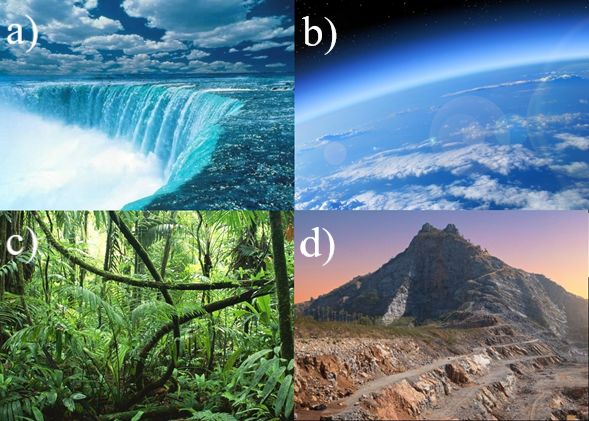
\includegraphics[scale=.8]{figuras/fig2.jpg}
	\caption{Ejemplo de las cuatro esferas de la tierra: a) hidrosfera; b) atm�sfera; c) biosfera; d) tierra s�lida.}
	
	\label{fig:fig2}
\end{figure}

La tierra solida se divide en tres capas la corteza, el manto y el n�cleo.  La corteza, capa rocosa externa, comparativamente fina de la Tierra, se divide generalmente en corteza oce�nica y corteza continental. El Manto representa m�s del 82 por ciento del volumen de la Tierra, una envoltura rocosa s�lida que se extiende hasta una profundidad de 2.900 kil�metros. El l�mite entre la corteza y el manto representa un cambio de composici�n qu�mica. N�cleo. Se cree que la composici�n del n�cleo es una aleaci�n de hierro y n�quel con cantidades menores de ox�geno, silicio y azufre, elementos que forman f�cilmente compuestos con el hierro (\cite{Lutgens2005}; \cite{rafferty2011geological}). En la Figura~\ref{fig:fig3} se detalla las subdivisiones de las  tres capas.

\begin{figure}[H]
	\centering
	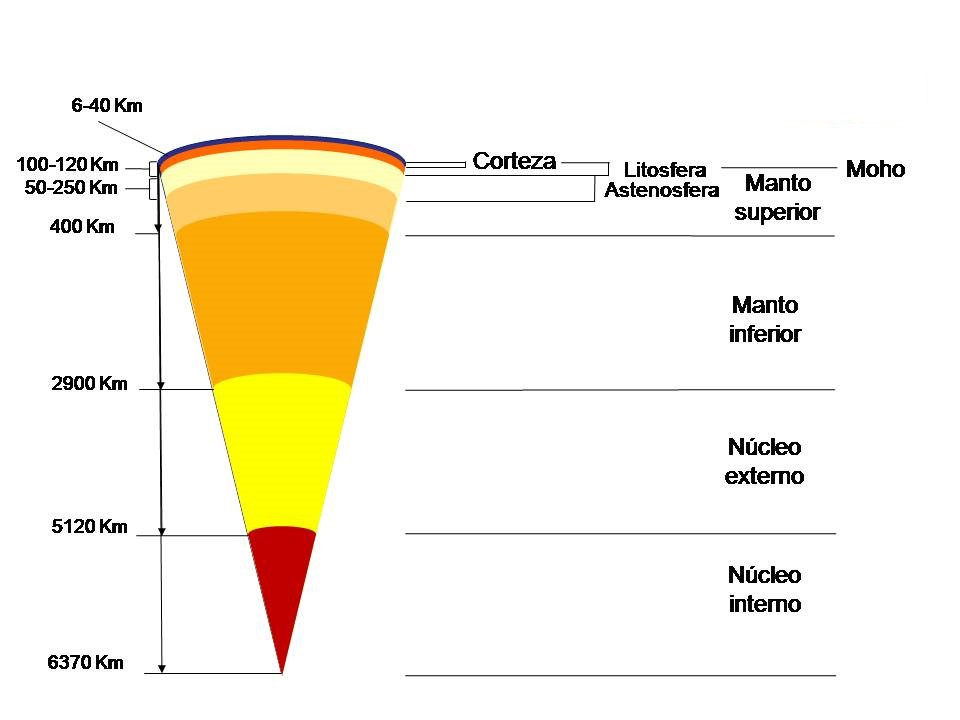
\includegraphics[scale=.5]{figuras/fig3.jpg}
	\caption{Estructura en capas de la Tierra.}
	\label{fig:fig3}
\end{figure}

De todas las capas existe un alto inter�s por la corteza ya que en ella se desvuelve la vida humana y la biosfera en general. Esta superficie terrestre es divida en continentes y las cuencas oce�nicas. Estas dos superficies tienen diferentes caracter�sticas f�sicas y qu�micas. Para la superficie terrestre continental el elemento fundamental de mayor abundancia son las rocas. Al examinar una roca con atenci�n, encontramos que consta de cristales o granos m�s peque�os denominados minerales. Los minerales son compuestos qu�micos (o en algunas ocasiones elementos �nicos), cada uno de ellos con su propia composici�n y sus propiedades f�sicas. La naturaleza de la roca est� definida por su composici�n qu�mica y por sus propiedades texturales (tama�o, forma y orientaci�n). Estos dos aspectos son reflejo de los procesos geol�gicos que la crearon. Esta comprensi�n tiene muchas aplicaciones pr�cticas, como en la b�squeda de recursos minerales y energ�ticos b�sicos y la soluci�n de problemas ambientales. 

\section{Las rocas y su ciclo}

Los ge�logos dividen las rocas en tres grandes grupos: �gneas, sedimentarias y metam�rfica, algunos ejemplos de cada tipo de roca se muestran en la Figura~\ref{fig:fig4}. Rocas �gneas. Las rocas �gneas (ignis = fuego) se forman cuando la roca fundida, denominada magma, se enfr�a y se solidifica. El magma es roca fundida que se puede formar a varios niveles de profundidad en el interior de la corteza de la Tierra y el manto superior. A medida que se enfr�a el magma, cristales de varios minerales se van formando y creciendo. Cuando el magma permanece en el interior profundo de la corteza, se enfr�a lentamente durante miles de a�os. Las rocas �gneas de grano grueso que se forman muy por debajo de la superficie se denominan plut�nicas. Las rocas �gneas que se forman en la superficie terrestre se denominan volc�nicas y suelen ser de grano fino. 

\begin{figure}[H]
	\centering
	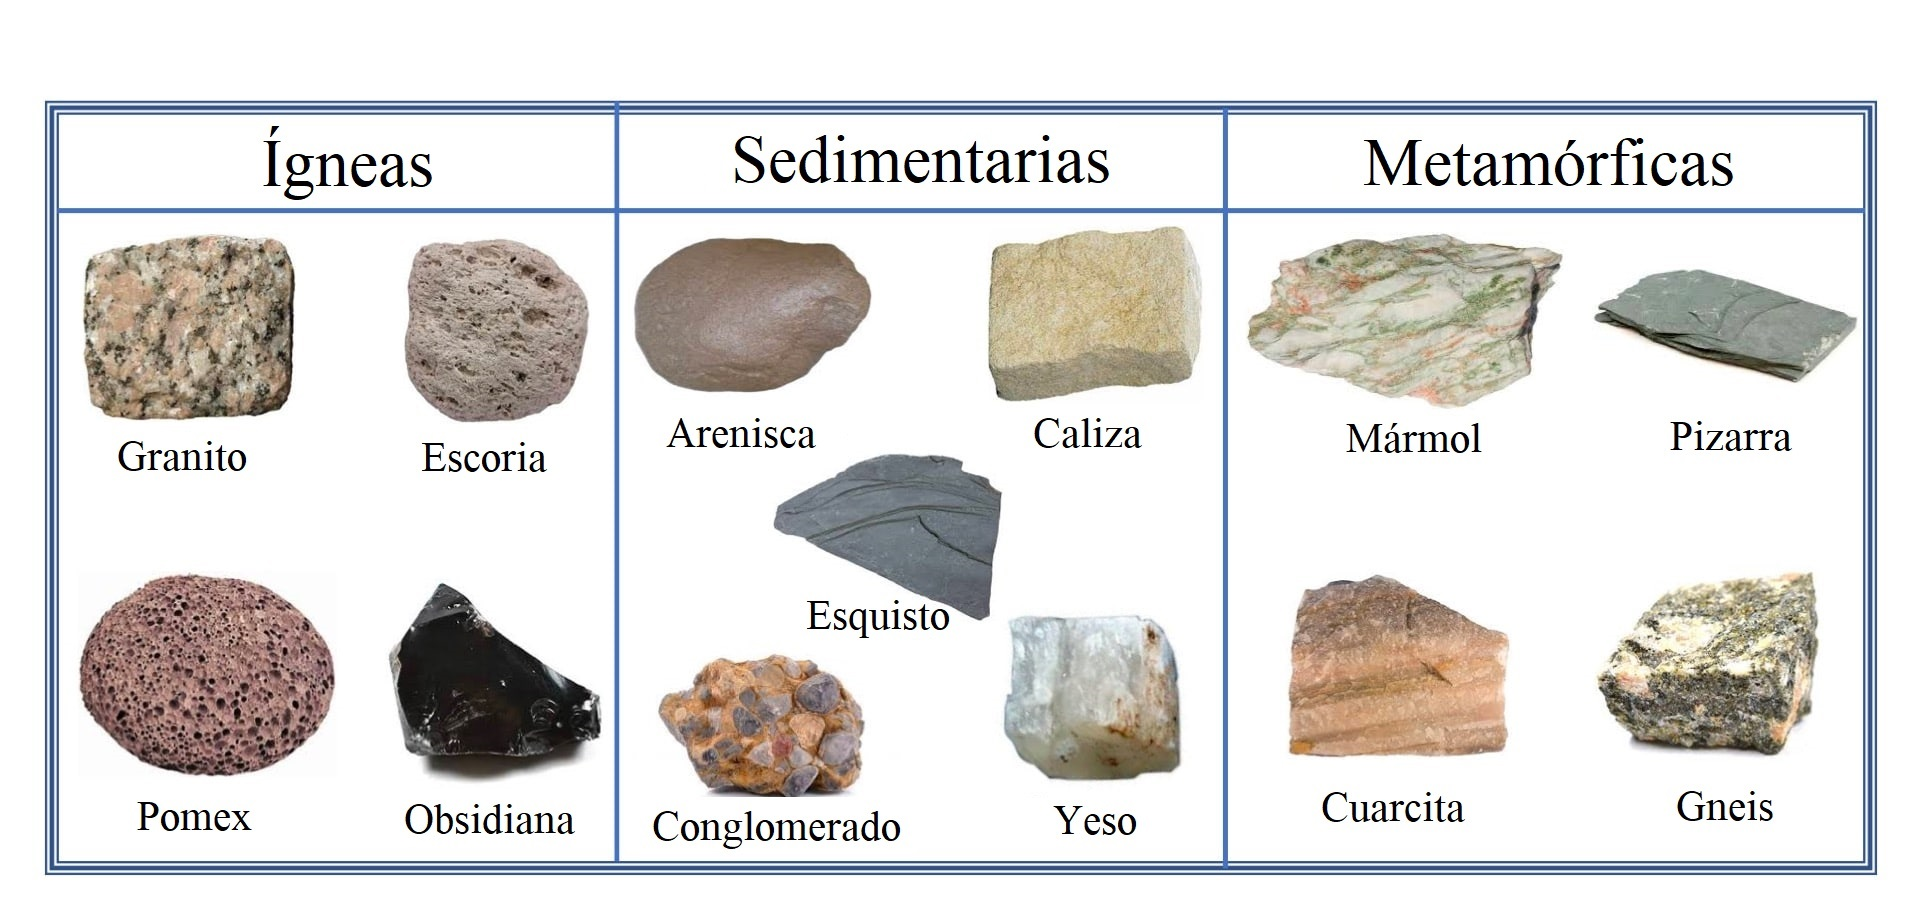
\includegraphics[scale=.4]{figuras/fig4.jpg}
	\caption{Ejemplos de los tres tipos de rocas.}
	
	\label{fig:fig4}
\end{figure}

%, en la Figura~\ref{fig:fig5} se muestra un tipo de sedimento
Las rocas sedimentarias se forman por acumulaci�n de sedimentos. Los sedimentos est�n compuestos de part�culas de diversos tama�os transportadas y son sometidos a procesos f�sicos y qu�micos (diag�nesis), que dan lugar a materiales consolidados. El agua, el viento o el hielo glacial suelen transportar los productos de la meteorizaci�n (fragmentaci�n de rocas) a lugares de sedimentaci�n donde �stos forman capas relativamente planas. Normalmente los sedimentos se convierten en roca o se litifican por la compactaci�n y cementaci�n. La compactaci�n tiene lugar a medida que el peso de los materiales suprayacentes comprime los sedimentos en masas m�s densas. La cementaci�n se produce conforme el agua que contiene sustancias disueltas se filtra a trav�s de los espacios intergranulares del sedimento. Con el tiempo, el material disuelto en agua precipita entre los granos y los cementa en una masa s�lida.

El tercer tipo son las rocas metam�rficas. Estas se producen a partir de rocas �gneas, sedimentarias o incluso otras rocas metam�rficas. As�, cada roca metam�rfica tiene una roca madre, la roca a partir de la que se ha formado. Metam�rfico es un adjetivo adecuado porque su significado literal es �cambiar la forma�. La mayor�a de cambios tienen lugar a temperaturas y presiones elevadas que se dan en la profundidad de la corteza terrestre y el manto superior. Los procesos que crean las rocas metam�rficas a menudo progresan de una manera incremental, desde cambios ligeros (metamorfismo de grado bajo) hasta cambios sustanciales (metamorfismo de grado alto).


%\begin{figure}[H]
%	\centering 
%	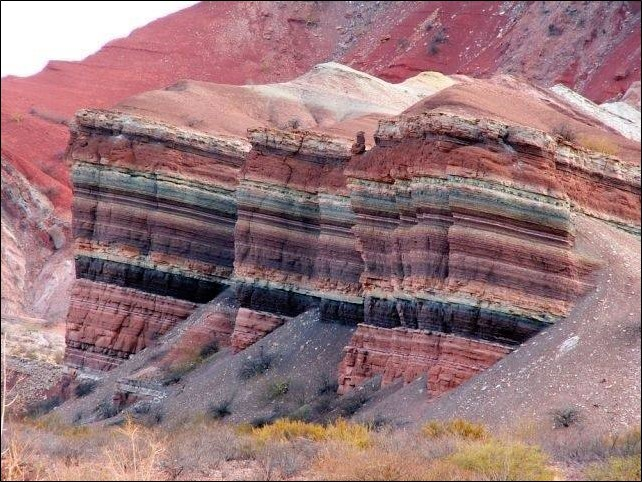
\includegraphics[scale=.7]{figuras/fig5.jpg}
%	\caption{Sedimento ubicado en M�tlili, en la provincia de Gharda�a, Argelia.}
%	\label{fig:fig5}
%\end{figure}

Estos tres tipos de rocas interact�an formando un ciclo, v�ase la Figura~\ref{fig:fig6}. Las rocas pueden pasar por cualquiera de los tres estados cuando son forzadas a romper el equilibrio. Una roca �gnea como el basalto puede disgregarse y alterarse cuando se expone a la atm�sfera, o volver a fundirse al subducir por debajo de un continente. Debido a las fuerzas generadoras del ciclo de las rocas, las placas tect�nicas y el ciclo del agua, las rocas no pueden mantenerse en equilibrio y son forzadas a cambiar ante los nuevos ambientes. 

Podemos iniciar explicando el ciclo con el magma. El magma que es la roca fundida que se forma a una gran profundidad por debajo de la superficie de la Tierra. Con el tiempo, el magma se enfr�a y se solidifica. Este proceso, denominado cristalizaci�n, puede ocurrir debajo de la superficie terrestre o, despu�s de una erupci�n volc�nica, en la superficie. En cualquiera de las dos situaciones, las rocas resultantes se denominan rocas �gneas.

\begin{figure}[H]
	
	\centering
	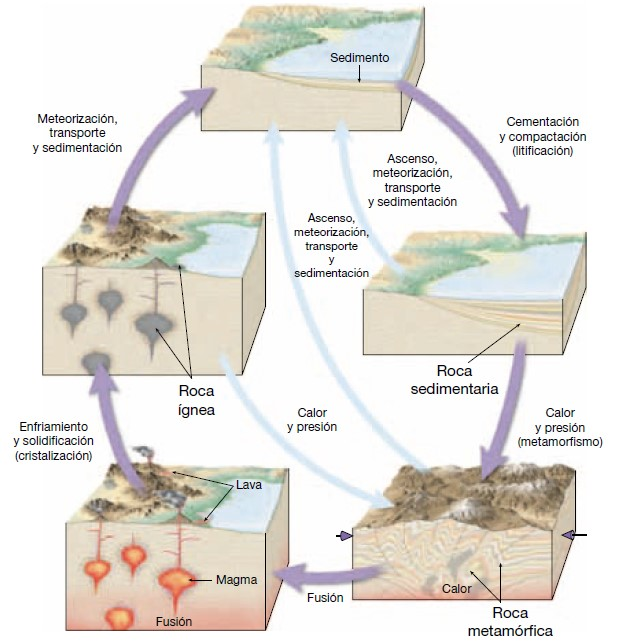
\includegraphics[scale=.85]{figuras/fig6.jpg}
	\caption{Ciclo de las rocas.}
	\label{fig:fig6}
\end{figure}

Si las rocas �gneas afloran en la superficie experimentar�n meteorizaci�n, en la cual la acci�n de la atm�sfera desintegra y descompone lentamente las rocas. Los materiales resultantes pueden ser desplazados pendiente abajo por la gravedad antes de ser captados y transportados por alg�n agente erosivo como las aguas superficiales, los glaciares, el viento o las olas. Por fin, estas part�culas y sustancias disueltas, denominadas sedimentos, son depositadas. Aunque la mayor�a de los sedimentos acaba llegando al oc�ano, otras zonas de acumulaci�n son las llanuras de inundaci�n de los r�os, los desiertos, los pantanos y las dunas. A continuaci�n, los sedimentos experimentan litificaci�n, un t�rmino que significa �conversi�n en roca�. El sedimento suele litificarse dando lugar a una roca sedimentaria cuando es compactado por el peso de las capas suprayacentes o cuando es cementado conforme el agua subterr�nea de infiltraci�n llena los poros con materia mineral. Si la roca sedimentaria resultante adquiere la profundidad necesaria dentro de la tierra, interact�a con una masa de magma, y estar� sometida a grandes presiones o a un calor intenso. La roca sedimentaria reaccionar� ante este ambiente y se convertir� en un tercer tipo de roca, una roca metam�rfica. Cuando la roca metam�rfica es sometida a cambios de presi�n adicionales o a temperaturas a�n mayores, se fundir�, creando un magma, que acabar� cristalizando en rocas �gneas. Los procesos impulsados por el calor desde el interior de la Tierra son responsables de la creaci�n de las rocas �gneas y metam�rficas. La meteorizaci�n y la erosi�n, procesos externos alimentados por una combinaci�n de energ�a procedente del Sol y la gravedad, producen el sedimento a partir del cual se forman las rocas sedimentarias. Caminos alternativos. Las v�as mostradas en el ciclo b�sico no son las �nicas posibles. Al contrario, es exactamente igual de probable que puedan seguirse otras v�as distintas de las descritas en la secci�n precedente. Esas alternativas se indican mediante las l�neas azules en la Figura~\ref{fig:fig6}. Las rocas �gneas, en vez de ser expuestas a la meteorizaci�n y a la erosi�n en la superficie terrestre, pueden permanecer enterradas profundamente. Esas masas pueden acabar siendo sometidas a fuertes fuerzas de compresi�n y a temperaturas elevadas asociadas con la formaci�n de monta�as. Cuando esto ocurre, se transforman directamente en rocas metam�rficas. Las rocas metam�rficas y sedimentarias, as� como los sedimentos, no siempre permanecen enterrados, por el contrario, las capas superiores pueden ser eliminadas, dejando expuestas las rocas que antes estaban enterradas. Cuando esto ocurre, los materiales son meteorizados y convertidos en nueva materia prima para las rocas sedimentarias. Las rocas pueden parecer masas invariables, pero el ciclo de las rocas demuestra que no es as�. Los cambios, sin embargo, requieren tiempo; grandes cantidades de tiempo.   

\section{Rocas sedimentarias}

Las rocas sedimentarias son de gran inter�s por las siguientes razones: (1) Cubren alrededor del 80\% de la corteza terrestre, que es la parte de la tierra s�lida con la que m�s interactuamos. (2) Representan la base del conocimiento de otras �reas geol�gicas como la estratigraf�a y la geolog�a estructural. (3) Un alto porcentaje de la actividad econ�mica est� relacionada con dep�sitos de rocas sedimentarias, algunos ejemplos son: el petr�leo, el gas natural, carb�n, sal, sulfuro, potasio, yeso, caliza, fosfato, uranio, hierro, magnesio y una numerosa lista de elementos en la construcci�n. (4) En la geotecnia son una parte importante para caracterizar el tipo de suelo. (5) En la petrolog�a sedimentaria es clave para determinar la litolog�a, relieve, clima y actividad tect�nica.     

Como se describi� anteriormente las rocas sedimentarias son resultante del dep�sito de material solido producto de la meteorizaci�n mec�nica y qu�mica. La transformaci�n del sedimento en roca sedimentaria se conoce como  litificaci�n. El sedimento puede experimentar grandes cambios desde el momento en que fue depositado hasta que se convierte en una roca sedimentaria y posteriormente es sometido a las temperaturas y las presiones que lo transforman en una roca metam�rfica. El t�rmino diag�nesis (d�a=cambio; g�nesis=origen) es un t�rmino general para todos los cambios qu�micos, f�sicos y biol�gicos que tienen lugar despu�s de la deposici�n de los sedimentos, as� como durante y despu�s de la litificaci�n. La litificaci�n se refiere a los procesos mediante los cuales los sedimentos no consolidados se transforman en rocas sedimentarias s�lidas (lithos=piedra; fic=hacer). Los procesos b�sicos de litificaci�n son la compactaci�n y la cementaci�n, v�ase la Figura~\ref{fig:fig7}.

\begin{figure}[H]
	\centering
	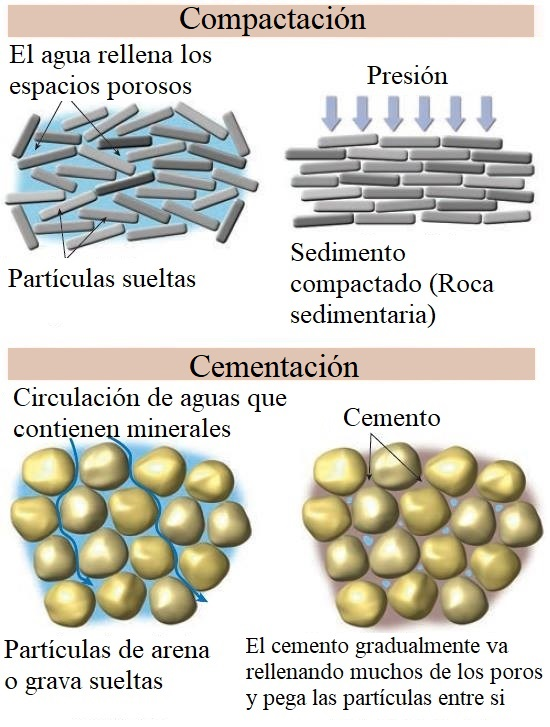
\includegraphics[scale=.85]{figuras/fig7.jpg}
	\caption{Formaci�n de rocas sedimentarias. Litificaci�n de sedimentos. Compactaci�n y cementaci�n.}
	\label{fig:fig7}
\end{figure}

El cambio diagen�tico f�sico m�s habitual es la compactaci�n. Conforme el sedimento se acumula a trav�s del tiempo, el peso del material suprayacente comprime los sedimentos m�s profundos. Cuanto mayor es la profundidad a la que est� enterrado el sedimento, m�s se compacta y m�s firme se vuelve. Al inducirse cada vez m�s la aproximaci�n de los granos, hay una reducci�n considerable del espacio poroso (el espacio abierto entre las part�culas). Conforme se reduce el espacio del poro, se expulsa gran parte del agua que estaba atrapada en los sedimentos. Dado que las arenas y otros sedimentos gruesos son s�lo ligeramente compresibles, la compactaci�n, como proceso de litificaci�n, es m�s significativa en las rocas sedimentarias de grano fino.  La cementaci�n es el proceso m�s importante mediante el cual los sedimentos se convierten en rocas sedimentarias. Es un cambio diagen�tico qu�mico que implica la precipitaci�n de los minerales entre los granos sedimentarios individuales. Los materiales cementantes son transportados en soluci�n por el agua que percola a trav�s de los espacios abiertos entre las part�culas. A lo largo del tiempo, el cemento precipita sobre los granos de sedimento, llena los espacios vac�os y une los clastos. De la misma manera que el espacio del poro se reduce durante la compactaci�n, la adici�n de cemento al dep�sito sedimentario reduce tambi�n su porosidad.

\begin{figure}[H]
	\centering
	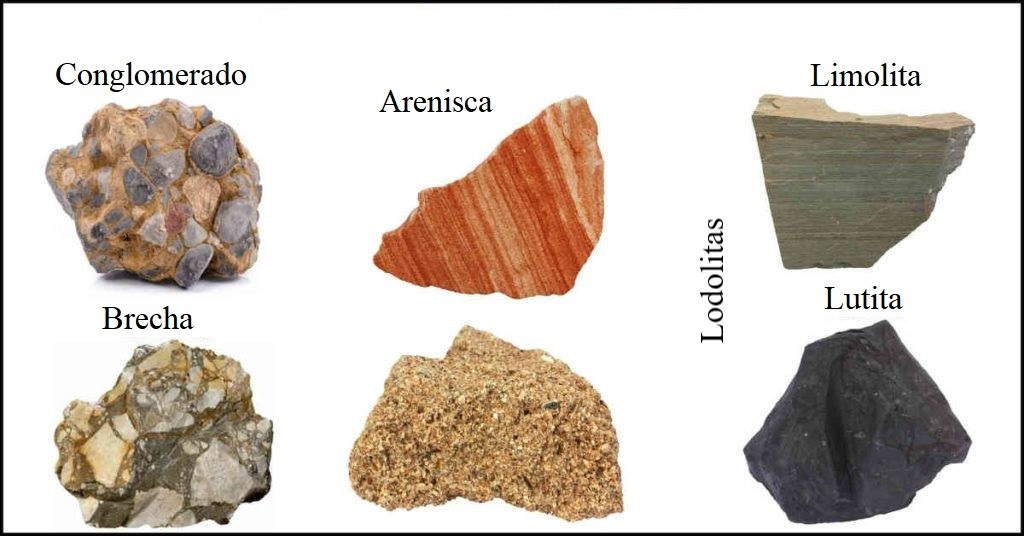
\includegraphics[scale=.5]{figuras/fig9.jpg}
	\caption{Rocas sedimentarias detr�ticas.}
	\label{fig:fig8}
\end{figure}

El sedimento tiene dos or�genes principales. En primer lugar, el sedimento puede ser una acumulaci�n de material que se origina y es transportado en forma de clastos s�lidos derivados de la meteorizaci�n mec�nica y qu�mica. Los dep�sitos de este tipo se denominan detr�ticos y las rocas sedimentarias que forman, rocas sedimentarias detr�ticas, como se muestra en la Figura~\ref{fig:fig8}.

La segunda fuente principal de sedimento es el material soluble producido en gran medida mediante meteorizaci�n qu�mica. Cuando estas sustancias disueltas son precipitadas mediante procesos org�nicos o inorg�nicos, el material se conoce como sedimento qu�mico y las rocas formadas a partir de �l se denominan rocas sedimentarias qu�micas, como se muestra en la Figura~\ref{fig:fig9}.

\begin{figure}[H]
	\centering
	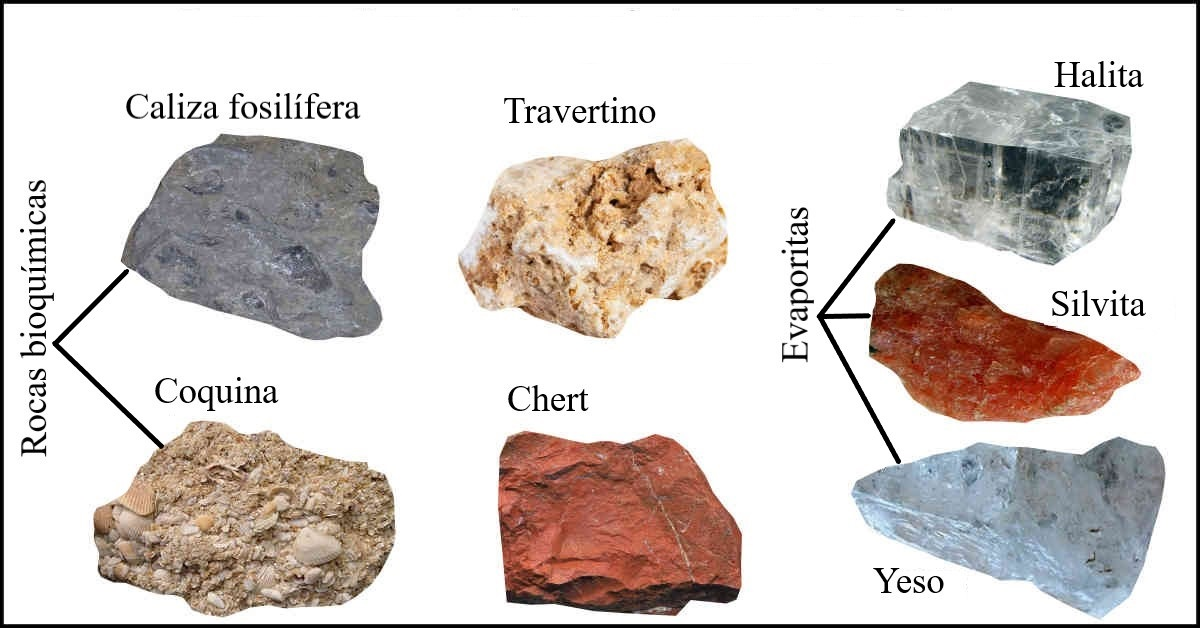
\includegraphics[scale=.4]{figuras/fig10.jpg}
	\caption{Rocas sedimentarias qu�micas.}
	\label{fig:fig9}
\end{figure}

\section{Morfolog�a de rocas sedimentarias}

El an�lisis de las rocas sedimentarias contempla aspectos f�sicos, qu�micos y mineral�gicos. Dentro de los f�sicos existen tres descriptores; el tama�o, la morfolog�a y la orientaci�n. El tama�o y la orientaci�n de la roca es un tema bien establecido. Sin embargo la morfolog�a es un tema relativamente reciente y se encuentra en desarrollo. %Meter una referencia

En la morfolog�a de la roca se graban la configuraci�n de la g�nesis, el ambiente, transporte y deposici�n. Por ejemplo, cuando las corrientes de agua, el viento o las olas mueven la arena y otros clastos sedimentarios, los granos pierden sus bordes y esquinas angulosos y se van redondeando m�s a medida que colisionan con otras part�culas durante el transporte. Por tanto, es probable que los granos redondeados hayan sido transportados por el aire o por el agua. Adem�s, el grado de redondez indica la distancia o el tiempo transcurrido en el transporte del sedimento por corrientes de aire o agua. Granos muy redondeados indican que se ha producido una gran abrasi�n y, por consiguiente, un prolongado transporte. Los granos muy angulosos, por otro lado, significan dos cosas: que los materiales sufrieron transporte durante una distancia corta antes de su dep�sito, y que quiz� los haya transportado alg�n otro medio. Por ejemplo, cuando los glaciares mueven los sedimentos, los clastos suelen volverse m�s irregulares por la acci�n de trituraci�n y molienda del hielo. Adem�s de afectar al grado de redondez y al grado de selecci�n que los clastos experimentan, la duraci�n del transporte a trav�s de corrientes de agua y aire turbulentas influye tambi�n en la composici�n mineral de un dep�sito sedimentario. Una meteorizaci�n sustancial y un transporte prolongado llevan a la destrucci�n gradual de los minerales m�s d�biles y menos estable. As� en la morfolog�a esta parte de la clave para reconstruir la historia y caracter�sticas de procesos sedimentarios.  


\section{Forma, redondez y rugosidad}

La morfolog�a de una roca sedimentaria puede ser descrita por tres componentes: la forma, la redondez y la rugosidad como se muestra en la Figura~\ref{fig:fig10} respectivamente. Estas propiedades son independientes entre s�, esto es que una puede variar sin afectar las otras dos. Estas tres propiedades se distinguen, al menos, por sus escalas. Esta caracter�stica permite ordenarlas de  manera jer�rquica, como se muestra en la Figura~\ref{fig:fig11}. La forma, propiedad de primer orden, refleja los grandes rasgos que tiene la part�cula; la redondez, propiedad de segundo orden, refleja los cambios en las esquinas. Estas variaciones se encuentran superpuestas en la forma. La rugosidad, propiedad de tercer orden, son las variaciones superpuestas en la superficie y en las esquinas \cite{BARRETT1980}.

\begin{figure}[H]
	
	\centering
	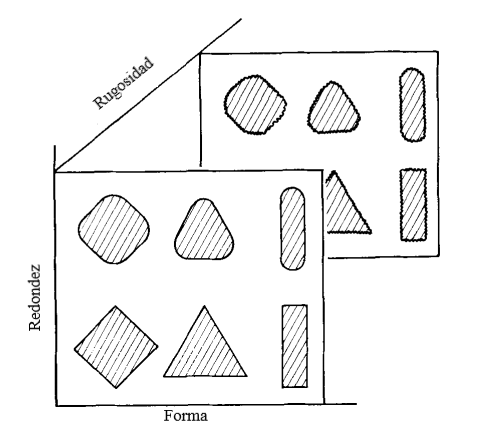
\includegraphics[scale=.7]{figuras/fig11.png}
	\caption{Una representaci�n simplificada de la forma, redondez y rugosidad en 3 dimensiones para ilustrar su independencia \cite{BARRETT1980}.}
	\label{fig:fig10}
\end{figure}

Este modo jer�rquico de la forma, redondez y rugosidad esta basado en los fenomenos geol�gico a los que se exponen las rocas. Cambios en la rugosidad no necesariamente afectan a la redondez. La meteorizaci�n puede aumentar la rugosidad de una roca, pero las esquinas muy redondeas se mantendr�n igual. Estr�as, quebraduras y otras caracter�sticas se pueden obtener sin cambiar la redondez. Esto no imposibilita que este proceso haga que la rugosidad cambie la redondez despu�s de un largo per�odo de tiempo. La redondez de una roca, puede incrementar a trav�s de la abrasi�n, sin afectar mucho a la forma. En contraste, un cambio en la forma inevitablemente afectar� a la redondez y rugosidad, porque las superficies nuevas son expuestas, y aparecer�an nuevas esquinas, y un cambio en la redondez deber�a afectar a la rugosidad, as� que por cada cambio resulta en una nueva morfolog�a \cite{BARRETT1980}.

\begin{figure}[H]
	
	\centering
	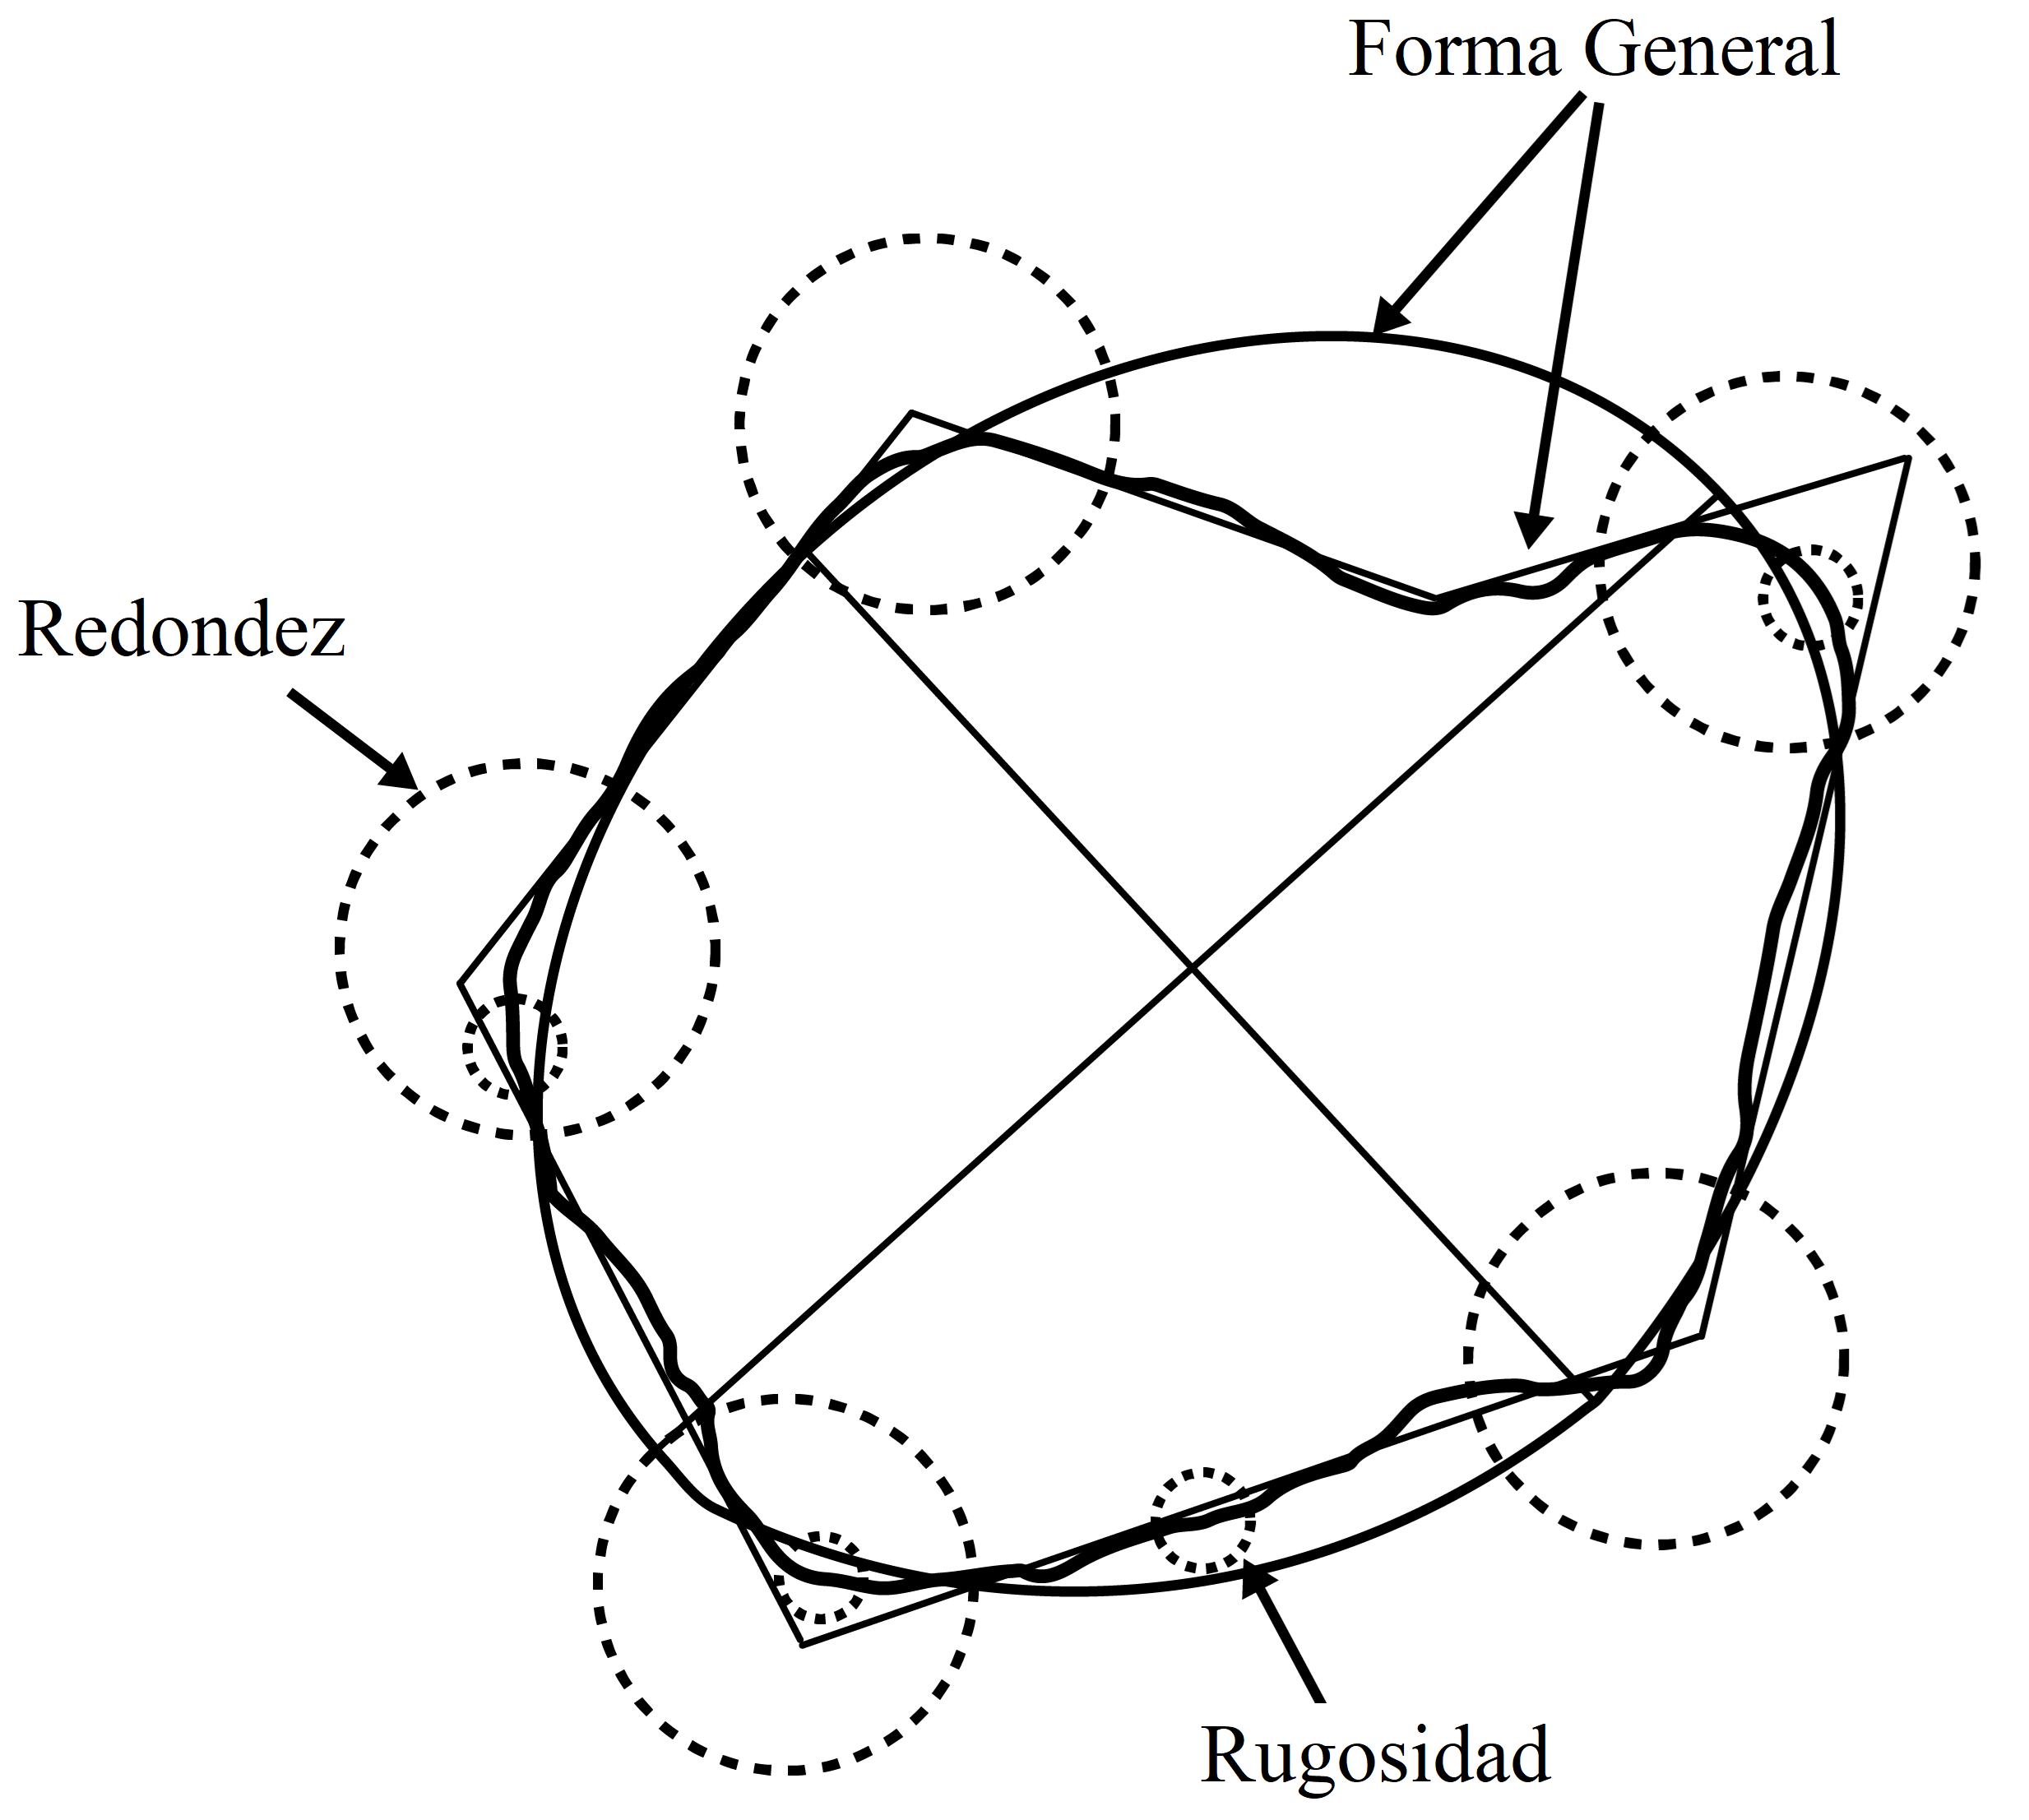
\includegraphics[scale=.2]{figuras/fig1.png}
	\caption{Forma, redondez y  textura superficial  propuestas por Barrett \cite{BARRETT1980}.}
	\label{fig:fig11}
\end{figure}


Existen definiciones y clasificaciones bien definidas para medir la forma y redondez. Por otro lado, en lo que respecta a la rugosidad no existe un acuerdo entre los cientificos, sin embargo hay algunos intentos de caracterizarla y medirla \cite{Rodriguez2013}.

El presente trabajo se enfoca a la medici�n de la forma y la redondez, dejando de lado la rugosidad por no existir a�n un consenso en su descripci�n. Los diferentes m�todos para medir la forma y redondez se discutir�n en los siguientes dos subsecciones.


\section{M�todos para obtener la forma}

El par�metro m�s �til para medir la forma es el grado de esfericidad. La esfericidad cuantifica el grado de similitud entre la part�cula y una esfera. Una de las m�tricas m�s usadas para medir la esfericidad es la propuesta por Wadell\cite{Wadell1932}, que define la esfericidad como la relaci�n entre el �rea de superficie de la esfera del mismo volumen y el �rea de la superficie real de la part�cula. Esta m�trica necesita las tres dimensiones de la part�culas, sin embargo existe su equivalente bidimensional \cite{Altuhafi2013}.

Las siguientes m�tricas representan las formas m�s comunes para medir la esfericidad en dos dimensiones son:
\begin{equation}
\text{Esfericidad por el �rea} \colon S_A = \frac{A_s}{A_{cir}}
\end{equation}
 donde \(A_s\) es el �rea proyectada de la part�cula y \(A_{cir}\) es el �rea del c�rculo m�nimo que inscribe a la part�cula, f�rmula propuesta por Tickell\cite{tickell1939examination}.
\begin{equation}
\text{Esfericidad por el di�metro} \colon S_D = \frac{d_c}{D_{cir}}
\end{equation}
 donde \(d_c\) es el di�metro del c�rculo igual en �rea que la part�cula normalizada cuya cara m�s larga descansa, es decir paralela al plano de los ejes largo e intermedio, y \(D_{cir}\) es el di�metro del c�rculo m�s peque�o que inscribe a la part�cula. Los rangos de valor de est� f�rmula est�n distribuidos de 0.54 a 1, propuesta por Wadell\cite{Wadell1935}.
\begin{equation}
\text{Esfericidad por la relaci�n de c�rculos} \colon S_C = \frac{D_{ins}}{D_{cir}}
\end{equation}
 donde \(D_{ins}\) es el di�metro del m�nimo c�rculo circunscrito en la part�cula y \(D_{cir}\) es el di�metro del c�rculo m�s peque�o que inscribe a la part�cula, f�rmula propuesta por Santamarina y Cho\cite{Santamarina2004}.
\begin{equation}
\text{Esfericidad por el Per�metro} \colon S_P = \frac{P_c}{P_s}
\end{equation}
donde \(P_c\) es el per�metro del c�rculo que tiene la misma �rea que la part�cula y \(P_s\) es el per�metro de la part�cula, f�rmula propuesta por Altuhafi \cite{Altuhafi2013}.
\begin{equation}
\text{Esfericidad por relaci�n entre anchura y altura} \colon S_{WL} = \frac{d_1}{d_2}
\end{equation}
donde \(d_1\) y \(d_2\) son el ancho y el largo de la part�cula respectivamente, f�rmula propuesta por Krumbein \cite{krumbein1951stratigraphy}.

Existen m�s definiciones para la esfericidad que se basan en el volumen, como la propuesta por Wadell \cite{wadell1933sphericity}, pero no se toman en cuenta porque en este trabajo las part�culas que ser�n caracterizadas son en dos dimensiones.

Para fines de este trabajo, la esfericidad que se usa es la propuesta por Wadell \cite{Wadell1935} para dos dimensiones, debido a que es una de las m�s conocidas y usadas para describir la forma de una part�cula.

\section{M�todos para obtener la redondez}
La redondez es un concepto que suele confundirse con propiedades de la forma, es por eso que su concepto debe ser aclarado (\cite{krynine19561}; \cite{sneed1958pebbles}). Como se mencion� anteriormente, la redondez es una propiedad superpuesta a la forma que estima  la suavidad (o angulosidad) superficial de la part�cula \cite{Resentini2018}.

Las tres formas m�s comunes para medir la redondez se basan en c�rculos circunscritos, espectro de Fourier, y fractales.

El m�todo basado en c�rculos circunscritos se basa en que el radio de curvatura de una esquina no puede ser mayor al radio del m�ximo c�rculo circunscrito en la part�cula, por lo que la redondez de una esquina puede ser expresada como \(\frac{r}{R}\), donde \(r\) es el radio de curvatura de la esquina y \(R\) es el radio del m�ximo c�rculo circunscrito \cite{Wadell1932}.

La redondez total de un s�lido en un solo plano (2 dimensiones) se obtiene usando la media de la redondez de cada una de las esquinas en ese plano. Por lo que la f�rmula queda as�:
\begin{equation}
\frac{\sum{\frac{r}{R}}}{N} = \text{Grado de redondez}
\end{equation}
donde \(\sum{\frac{r}{R}}\) es la sumatoria de los valores de redondez de cada esquina, y \(N\) es el n�mero de esquinas de la part�cula en el plano dado. El m�ximo valor de redondez que puede ser obtenido es de \(1\). Este m�todo fue desarrollado por Wadell\cite{Wadell1932}. 


En el m�todo basado en la transformada de Fourier, el contorno de la part�cula se mapea a una funci�n uni o multivariable. A esta funci�n se aplica la transformada de Fourier. Esta transformaci�n permite separar las componentes de la morfolog�a en bandas frecuenciales, por lo que supone un procesamiento m�s sencillo para reconocer la forma, redondez y textura. Generalmente, la informaci�n esta contenida en la magnitud del espectro, dejando fuera la fase, haciendo que el m�todo sea invariante a la rotaci�n y traslaci�n. La invarianza a la escala es lograda normalizando la magnitud del espectro. 


%Completar este parrafo
La geometr�a basada en fractales es tambi�n otro buen m�todo para clasificar la redondez (\cite{kaye1978specification}, \cite{orford1983use}, \cite{sarocchi201117}). La t�cnica m�s usada para analizar los l�mites de las part�culas es conocido como \textit{"Structured Walk"}. En est� t�cnica, las irregularidades en el per�metro de una part�cula est�n relacionadas con la dimensi�n de fractal, la cual es estimada para superfecias de clastos en tres dimensiones por pol�gonos o segmentos de linea. Los lados de el pol�gono incrementan progresivamente. La dimensi�n de fractal es calculada por la pendiente de la l�nea que mejor se ajusta. Las limitaciones de este m�todo son, como la identificaci�n de los l�mites de una part�cula relacionada a el proceso de abrasi�n, y la sensibilidad a la difuminaci�n y el ruido de la imagen, son descritas por Leavers\cite{leavers2000use} y Stachowiak\cite{stachowiak1998numerical}. Informaci�n obtenida en \cite{chavez2020method}.


\section{Clasificaci�n de redondez de rocas sedimentarias}

Desde un punto de vista pr�ctico, no es suficiente solo medir el grado de redondez sino tambi�n clasificarla. Una herramienta muy usada por los sedimentologos para clasificar la morfolog�a de clastos es un gr�fico visual comparativo. Russell, Taylor y Pettijohn \cite{muller1967methods} desarroll� un gr�fico visual comparativo de un conjunto de referencias de part�culas de la redondez conocidas. Este gr�fico ofrec�a un manera f�cil y r�pida para estimar la redondez de part�culas en dos dimensiones. The Russell, Taylor y Pettijohn (RTP) referenciaban la figura con veinticinco part�culas organizadas en cinco diferentes categor�as de redondez; angular, sub-angular, sub-redondeada, redondeada y bien redondeada \cite{Boggs2013}. En la Figura~\ref{fig:fig12}, las clasificaciones en filas corresponden a las de la redondez y las clasificaciones por columna son la esfericidad.

\begin{figure}[H]
	\centering
	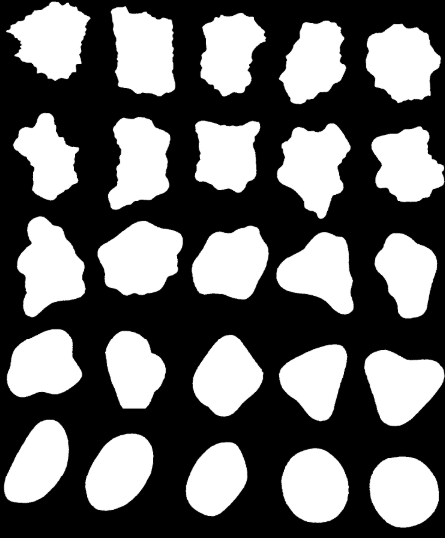
\includegraphics[scale=.6]{figuras/fig12.png}
	\caption{Clasificaciones para la redondez de una part�cula propuestas por Russell, Taylor y Pettijohn \cite{muller1967methods}.}
	\label{fig:fig12}
\end{figure}

Adem�s de la propuesta Russell, Taylor y Pettijohn, existe tambi�n la propuesta que hizo Krumbein, en la Figura~\ref{fig:fig13}, se observa que el clasifica el t�rmino de redondez en nueve clases, muy utilizada tambi�n.

\begin{figure}[H]
	
	\centering
	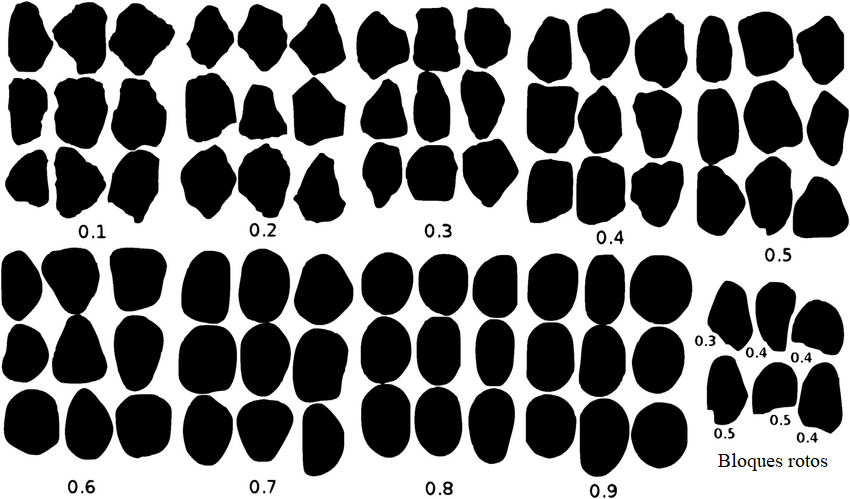
\includegraphics[scale=.7]{figuras/fig13.png}
	\caption{Clasificaciones para la redondez de una part�cula propuestas por Krumbein\cite{Krumbein1941}.}
	\label{fig:fig13}
\end{figure}

El m�todo a utilizar para estimar la redondez, que ser� utilizada como valor objetivo en la red neuronal, va a ser el propuesto por Wadell\cite{Wadell1932}, debido a su simplicidad con respecto a los m�todos basados en Fourier y Fractales. Las clasificaci�n que se utilizar� ser� la de Krumbein y Sloss \cite{Krumbein1941} debido a su amplio uso en el campo geol�gico.

%\section{Modelo o esquema general de investigaci�n}
%Este trabajo tiene un enfoque de investigaci�n de tipo Aplicada, ya que busca la manera de crear un modelo de redes neuronales junto con el espectro de Fourier %El�ptico de las rocas sedimentarias. El modelo que se busca debe de ser preciso, r�pido y f�cil de usar, adem�s, que sea invariante a la escala, rotaci�n y traslaci�n.
 









































%\section{Modelos Ocultos de Markov}
%A continuacion abordaremos la teor�a de los Modelos Ocultos de Markov, que ha demostrado
%ser la que mejores resultados produce a la hora de implementar reconocedores de voz. Los introducimos
%a partir de los procesos m�s sencillos, a los que iremos a�adiendo elementos para obtener los
%modelos finales. Gran parte de este tema se dedica a resolver anal�ticamente los problemas
%fundamentales que se presentar�n al intentar aplicar estas ideas al reconocimiento de voz.
%
%\subsection{Procesos de Markov}
%\subsubsection{Definici�n}
%Un proceso de Markov es un proceso aleatorio {q (n)} discreto en el tiempo, con la particularidad
%de que la probabilidad del valor de cada muestra s�lo depende del valor de la anterior:
%
%\begin{figure}[H]
%\centering 
%\includegraphics[scale=.7]{mark.PNG}
%%\caption{Diagrama preprocesado de la se�al}
%\label{fig3}
%\end{figure}
%
%Se usar� la notaci�n [q\_{n}] = q (n) para denotar al estado del proceso en el instante n o muestra
%n -�sima , pues resume la informaci�n que toda la historia del proceso aporta al futuro del
%mismo.
%
%\textbf{Ejemplo}
%Un modelo AR(1) (Autorregresivo de orden 1) es un proceso de Markov:
%
%\begin{figure}[H]
%\centering 
%\includegraphics[scale=.7]{mark2.PNG}
%%\caption{Diagrama preprocesado de la se�al}
%\label{fig3}
%\end{figure}
%
%\subsection{Probabilidad de una secuencia concreta}
%Para calcular ahora la probabilidad de una secuencia concreta de muestras, debemos primero obtener el siguiente resultado v�lido para cualquier proceso aleatorio discreto.
%
%Sea {q=o... hasta la e-nesima} una secuencia concreta, obtenida al observar el proceso aleatorio
%{ } n q durante T muestras. Utilizando el Teorema de Bayes, podemos descomponer la probabilidad
%de obtener esa secuencia en t�rminos de un producto de las probabilidades de cada muestra,
%condicionadas por las muestras pasadas:
%
%\begin{figure}[H]
%\centering 
%\includegraphics[scale=.7]{mark3.PNG}
%%\caption{Diagrama preprocesado de la se�al}
%\label{fig3}
%\end{figure}
%
%Siempre se puede descomponer de la siguiente forma:
%\begin{figure}[H]
%\centering 
%\includegraphics[scale=.7]{mark4.PNG}
%%\caption{Diagrama preprocesado de la se�al}
%\label{fig3}
%\end{figure}
%
%Si seguimos descomponiendo, se puede inducir: 
%\begin{figure}[H]
%\centering 
%\includegraphics[scale=.7]{mark5.PNG}
%%\caption{Diagrama preprocesado de la se�al}
%\label{fig3}
%\end{figure}
%
%Los modelos anteriormente vistos son demasiado restrictivos para aplicarlos a una gran variedad
%de problemas de inter�s, puesto que cada estado se corresponde con un evento f�sico observable.
%Podemos extender el concepto de modelo de Markov para incluir el caso en el que la observaci�n
%es aleatoria, dependiente del estado en el que se encuentra el sistema.
%El modelo resultante se conoce como Modelo Oculto de Markov (HMM), y es un proceso
%doblemente estoc�stico con:
%
%\begin{itemize}
%\item Un proceso estoc�stico subyacente que no es observable (est� oculto), sino que s�lo puede
%ser observado a trav�s de otro proceso (que s� es observable). Conforma la secuencia de
%estados por la que pasa el sistema.
%\item Un conjunto de procesos estoc�sticos que producen la secuencia de observaci�n.
%\end{itemize}
%
%Por lo tanto, un Modelo Oculto de Markov es una cadena de Markov en la que la observaci�n no
%es la propia secuencia de estados (que permanece oculta), sino que es el resultado de ciertos
%procesos estoc�sticos que se producen en cada estado.
%
%\subsection{Elementos de un Modelo Oculto de Markov}
%
%Un modelo oculto de Markov esta caracterizado por: 
%
%\begin{itemize}
%\item El n�mero de estados en el modelo (N ). Aunque los estados est�n ocultos, para muchas
%aplicaciones pr�cticas hay un significado f�sico asociado a los estados del modelo.
%Normalmente los estados est�n interconectados tal que cada uno puede ser alcanzado
%desde cualquier otro estado (modelo erg�dico). Sin embargo, como veremos m�s tarde,
%existen otros tipos de conexi�n entre estados que resultar�n de inter�s en el caso
%concreto del reconocimiento de voz.
%
%\item El n�mero de s�mbolos distintos observables en cada estado (M), es decir, el tama�o
%del alfabeto. Aqu�, los s�mbolos observados corresponden con la salida f�sica del sistema.
%
%\item La distribuci�n de probabilidades de transici�n entre estados ( A ).
%
%\item La distribuci�n de probabilidades de los s�mbolos observados en el estado.
%
%\item La distribuci�n inicial de estados.
%\end{itemize}
%
%\subsubsection{Representacion mediante rejilla}
%
%Podemos a�adir elementos a la representaci�n del trellis para modelar HMMs:
%
%\begin{itemize}
%\item Probabilidades iniciales de cada estado.
%\item Probabilidades de observaci�n de s�mbolos en cada estado.
%\end{itemize}
%
%\begin{figure}[H]
%\centering 
%\includegraphics[scale=.8]{trellis.PNG}
%%\caption{Diagrama preprocesado de la se�al}
%\label{fig3}
%\end{figure}
%
%\section{Modelado del Habla para el reconocimiento de voz}
%
%\subsection{Fundamentos}
%Para el reconocimiento de palabras aisladas, los modelos ocultos de Markov han demostrado en
%aplicaciones pr�cticas ser aquellos que mejores resultados producen. La idea es asignar a cada
%posible palabra del vocabulario (de tama�o W ) un modelo de estructura similar pero de
%diferentes par�metros:
%
%\begin{figure}[H]
%\centering 
%\includegraphics[scale=.7]{mark6.PNG}
%%\caption{Diagrama preprocesado de la se�al}
%\label{fig3}
%\end{figure}
%
%Cada modelo est� formado por distintos estados, en los cuales se generan los s�mbolos que
%constituyen la secuencia de observaci�n. Por otro lado, cada palabra est� formada por distintos
%fonemas. La relaci�n entre estados y fonemas no es directa y ser� abordada m�s adelante. La
%secuencia de estados es desconocida a priori:
%
%\begin{figure}[H]
%\centering 
%\includegraphics[scale=.7]{mark7.PNG}
%%\caption{Diagrama preprocesado de la se�al}
%\label{fig3}
%\end{figure}
%
%Por �ltimo la palabra recibida (y que queremos reconocer) se corresponder�, despu�s de un
%an�lisis que extrae sus caracter�sticas m�s importantes (MFCC), con la secuencia observada. �sta
%es conocida en las etapas de entrenamiento, validaci�n y reconocimiento.
%
%\subsection{Procedimiento para el modelado}
%
%Consideremos el siguiente reconocedor de palabras aisladas. Para cada palabra de un vocabulario
%(de W palabras) queremos dise�ar un HMM diferente, de N estados. Representamos la se�al de
%voz de una palabra dada como una secuencia discreta de vectores que codifican las
%caracter�sticas esenciales de la palabra: los coeficientes MFCC.
%
%La primera tarea es construir modelos individuales para cada palabra, usando la soluci�n al
%problema 3 para estimar los par�metros �ptimos.
%
%Para la comprensi�n del significado f�sico de los estados del modelo, usamos la soluci�n al
%problema 2. Con esto conseguimos segmentar cada modelo en estados, y entonces estudiar las
%propiedades de los vectores de observaci�n. El objetivo es refinar el modelo para mejorar su
%capacidad de modelar la secuencia recibida.
%
%Finalmente, una vez el conjunto de W modelos han sido dise�ados y optimizados, el
%reconocimiento de una palabra se realiza usando la soluci�n al problema 1. Se asigna una
%puntuaci�n a cada modelo basada en la secuencia observada de entrada, y se elige como palabra
%reconocida aquella cuya puntuaci�n sea m�xima.
%
%En la pr�ctica, la verosimilitud puede computarse a trav�s de la secuencia de estados m�s
%probable (problema 2), sin recurrir al c�lculo minucioso de todas las combinaciones posibles
%(problema 1).
%
%
%
%\section{Trabajos Relacionados}
%
%Dentro de la literatura que se ha estado recolectando para la escritura de esta tesis se ha encontrado un gran avance en cuanto a los Sistemas de Reconocimiento Autom�tico del Habla, los cuales se listan a continuaci�n y mas adelante ser�n abordados cada uno de ellos mas profundamente y obtener la informaci�n mas relevante que ayude al desarrollo de este trabajo de tesis. 
%
%\begin{itemize}
%\item Algoritmos y M�todos para el Reconocimiento de Voz en Espa�ol Mediante S�labas (2006)
%\item Reconocimiento de Voz Usando HTK (Universidad de Sevilla)
%\item Sistema de control activado por voz para uso en domotica (Enero 2016)
%\item Aplicaciones en reconocimento de voz utilizando HTK (Bogota, 2005)
%\item Modelo Ac�stico y de Lenguaje del Idioma Espa?nol para el dialecto Cucute?no, Orientado al Reconocimiento Automatico del Habla (2017)
%\item Reconomiento de Voz de ni�os para el espa�ol hablado en Mexico usando SONIC
%\item Un programa de reconocimiento de voz ayuda a los ni�os a aprender a leer (2004)
%\item El reconocimiento de voz mejora el rendimiento escolar de los ni�os con dislexia (2017)
%\item Implementaci�n de un m�dulo de reconocimiento de voz para ni�os mediante el procesamiento de se�ales aplicado en un caso pr�ctico (2017)\
%\item Efectos de un sistema de reconocimiento de voz en la conciencia fonol�gica y las
%habilidades de lectura de ni�os preescolares espa�oles (2016)
%\item Usabilidad en sistemas l�dicos infantiles con reconocimiento de voz como apoyo en la terapia de
%rehabilitaci�n de ni�os con problemas de lenguaje (2008)
%\item Reconocimiento de Voz para Ni�os con Discapacidad en el Habla (2004)
%
%\end{itemize}





       % incluye al archivo cuerpo_tesis.tex
\chapter{Modelo y propuesta de Investigaci�n}

\section{Modelo de Investigaci�n para la estimaci�n de par�metros morfol�gicos en rocas sedimentarias usando Fourier El�ptico y redes neuronales}

En la Figura~\ref{fig:fig14} se describen las etapas de investigaci�n, para despu�s ser detalladas.

\begin{itemize}
	\item La primera etapa consiste en conseguir 1123 im�genes de todas las clases de esfericidad y redondez para poder entrenar de manera balanceada la red, y despu�s probar con las im�genes de Krumbein (\cite{Krumbein1941}) para verificar las mediciones.
	
	\item La segunda etapa se obtiene el valor de redondez y esfericidad de cada una de las im�genes de entrenamiento con los m�todos propuestos.
	\item La tercera etapa consiste en calcular los primeros 40 arm�nicos de la serie de Fourier el�ptico de cada una de las im�genes de entrenamiento y relacionar estos arm�nicos con su valor de esfericidad y redondez.
	\begin{figure}[hbtp]
		\centering 
		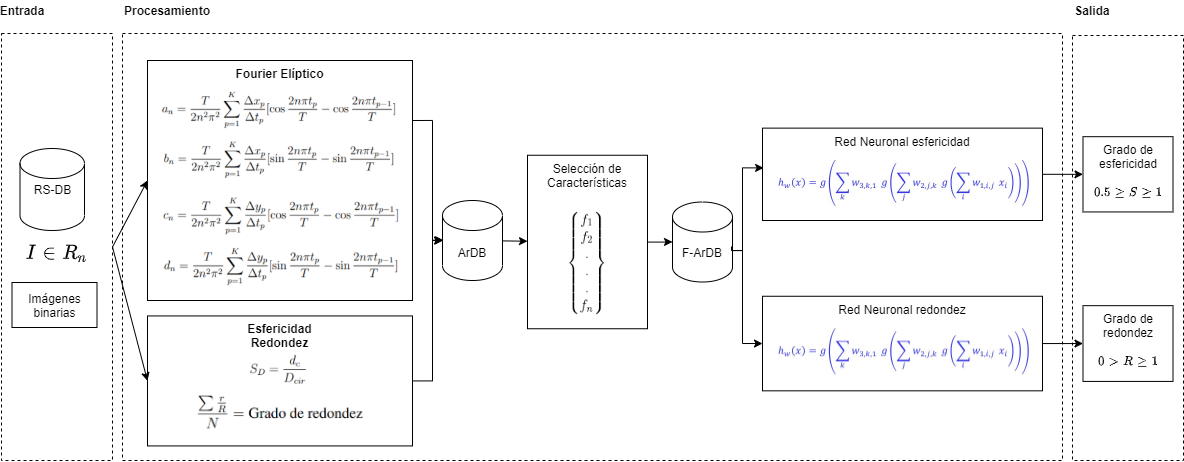
\includegraphics[angle=90,origin=c,scale=.55]{figuras/diagramaFlujoTrabajo.png}
		\caption{Modelo metodol�gico de la estimaci�n de par�metros morfol�gicos en rocas sedimentarias usando Fourier El�ptico y redes neuronales}
		\label{fig:fig14}
	\end{figure}
	\item La cuarta etapa consiste entrenar las 2 redes neuronales, la que clasifica la esfericidad, y la de la redondez, con los valores de entrada que ser�n los arm�nicos de Fourier El�ptico  y la su respectiva salida.
	\item Una vez entrenadas las redes, se prueban utilizando arm�nicos de Fourier El�ptico del conjunto de im�genes de prueba.
	
	\item La �ltima etapa es medir el error y clasificar las im�genes de prueba y observar los resultados.
\end{itemize}

\section{Fourier El�ptico}

El an�lisis de Fourier ha sido utilizado para caracterizar contornos cerrados. Fourier El�ptico es una extensi�n de Fourier cl�sico el cual simplifica la estimaci�n de los coeficientes a trav�s del c�digo de cadena del contorno cerrado. Los coeficientes correspondientes a la magnitud son invariantes a la escala, rotaci�n y traslaci�n.

El c�digo de cadena es el primer paso, inicialmente  descrito por Freeman\cite{freeman1974computer}, aproximando un contorno cerrado por una secuencia de trayectorias con 8 posibles valores. El c�digo de un contorno es la cadena \(V\) de longitud \(K\):
\begin{equation}
	V = a_1a_2a_3...a_K,
\end{equation}
donde cada uni�n \(a_i\) es un entero del 0 al 7 orientado en la direcci�n \((\frac{\pi}{r})a_i\) \cite{Kuhl1982}.
%Aclarar este parrafo
En la Figura~\ref{fig:fig15} se puede observar como un contorno cerrado separado en p�xeles, se puede obtener el c�digo de cadena, trazando una trayectoria desde un punto inicial, hasta volver a llegar a ese mismo punto, pasando por todo el contorno. El c�digo de cadena de la Figura~\ref{fig:fig15}a iniciando de el extremo superior izquierdo es:
\begin{equation}
	V = 0005676644422123
\end{equation}
\begin{figure}[H]
	\centering 
	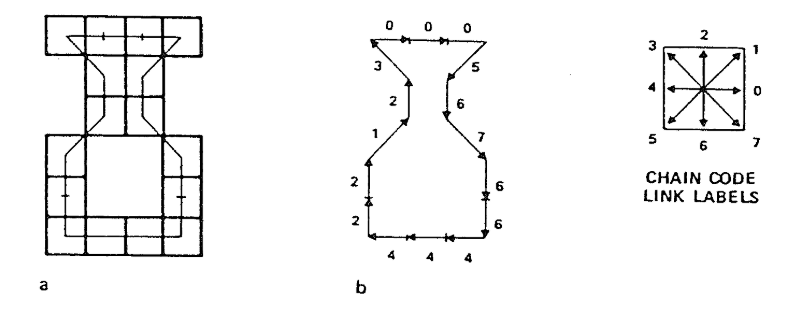
\includegraphics[scale=1]{figuras/codigoCadena.png}
	\caption{Representaci�n gr�fica del c�digo de cadena de un contorno cerrado \cite{Kuhl1982}}
	\label{fig:fig15}
\end{figure}

Debido a que el cambio en el c�digo de cadena esa constante, los coeficientes pueden ser encontrados m�s f�cilmente. Por lo que los coeficientes de la componente \(x\) son:
\begin{equation}
	a_n = \frac{T}{2n^2\pi^2}\sum_{p = 1}^{K}\frac{\Delta x_p}{\Delta t_p}[\cos{\frac{2n\pi t_p}{T}} - \cos{\frac{2n\pi t_{p-1}}{T}}]
\end{equation}
\begin{equation}
	b_n = \frac{T}{2n^2\pi^2}\sum_{p = 1}^{K}\frac{\Delta x_p}{\Delta t_p}[\sin{\frac{2n\pi t_p}{T}} - \sin{\frac{2n\pi t_{p-1}}{T}}]
\end{equation}
donde, la K es el n�mero de p�xeles del contorno, \(T\) el per�odo fundamental, \(\Delta x_p\) el cambio en el eje de las x, \(\Delta t_p\) el cambio en el tiempo.

Con eso obtendr�amos los coeficientes de la componente \(x\), pero como una imagen es una se�al en dos dimensiones, adem�s el cambio de la \(x\) no siempre sera igual al cambio en las \(y\), necesitamos tambi�n obtener los coeficientes de la componente \(y\).
\begin{equation}
	c_n = \frac{T}{2n^2\pi^2}\sum_{p = 1}^{K}\frac{\Delta y_p}{\Delta t_p}[\cos{\frac{2n\pi t_p}{T}} - \cos{\frac{2n\pi t_{p-1}}{T}}]
\end{equation}
\begin{equation}
	d_n = \frac{T}{2n^2\pi^2}\sum_{p = 1}^{K}\frac{\Delta y_p}{\Delta t_p}[\sin{\frac{2n\pi t_p}{T}} - \sin{\frac{2n\pi t_{p-1}}{T}}]
\end{equation}
Las cuatro expresiones anteriores conforman los coeficientes de Fourier el�ptico. Cabe notar que su nombre se debe a que genera fasores el�pticos en lugar de circulares como el m�todo tradicional.

Para que este m�todo obtenga la invarianza a la escala, rotaci�n y traslaci�n, es necesario aplicar una normalizaci�n y ajustar los �ngulos en los que va a iniciar cada elipse, para que independientemente de estas tres caracter�sticas del contorno cerrado siempre de el mismo resultado. La expresi�n para normalizar es la siguiente
\begin{equation}
	E_p = ((A_0-x_p)^2 + (C_0-y_p)^2)^\frac{1}{2}
\end{equation}
donde \(A_0\) y \(C_0\) son el promedio de la energ�a de las componentes \(x\) y \(y\) respectivamente. Para obtener el �ngulo de rotaci�n inicial \(\theta_p\) a el �ndice \(p\):
\begin{equation}
	\theta_p = \frac{2\pi t_p}{T}, 0<\theta_p\le2\pi
\end{equation}
y para obtener el �ngulo de rotaci�n espacial \(\psi_p\)
\begin{equation}
	\psi_p=\arctan[\frac{y_p-C_0}{x_p-A_0}], 0\le\psi_p<2\pi
\end{equation}
Al iniciar el c�lculo de los coeficientes, se tendr�a que obtener \(E_1\), \(\theta_1\) y \(\psi_1\) para influir en los siguiente coeficientes a que se reajusten de acuerdo a estos �ngulos iniciales, y dividirlo entre \(E_0\) para mantener la invarianza a la escala, por lo que la obtenci�n de los nuevos coeficientes ser�a:
\begin{equation}
	\begin{bmatrix}
	1a^{**}_n & 1b^{**}_n\\
	1c^{**}_n & 1d^{**}_n
	\end{bmatrix} =
	\begin{bmatrix}
	\cos{\psi_1} & \sin{\psi_1}\\
	-\sin{\psi_1} & \cos{\psi_1}
	\end{bmatrix}
	\begin{bmatrix}
	a_n & b_n\\
	c_n & d_n
	\end{bmatrix}
	\begin{bmatrix}
	\cos{n\theta_1} & -\sin{n\theta_1}\\
	\sin{n\theta_1} & \cos{n\theta_1}
	\end{bmatrix}
\end{equation}
\begin{equation}
	\begin{bmatrix}
	2a^{**}_n & 2b^{**}_n\\
	2c^{**}_n & 2d^{**}_n
	\end{bmatrix} =
	(-1)^{n+1}
	\begin{bmatrix}
	1a^{**}_n & 1b^{**}_n\\
	1c^{**}_n & 1d^{**}_n
	\end{bmatrix}
\end{equation}
El resultado de la ecuaci�n 3.11 nos dar�a los coeficientes \(a,b,c,d\) para el \(n\) arm�nico que se est� calculando. Siendo invariante a la escala, rotaci�n y traslaci�n. Los detalles pueden ser consultados en \cite{Kuhl1982}.
\section{Algoritmo para estimar la redondez}

El t�rmino de redondez es una caracter�stica morfol�gica m�s compleja que la forma. Se dice que es de segundo orden porque esta superpuesta a la forma, esto la hace independiente. Como mencionamos anteriormente, la redondez se medir� mediante la m�trica propuesta de Wadell \cite{Wadell1935} que consiste en identificar las principales curvaturas (esquinas) del contorno. El concepto es simple pero su algoritmo es complejo debido a que el n�mero y grado de curvatura depende del tama�o del contorno. Proponemos utilizar el algoritmo desarrollado por Zheng \cite{Zheng2016} el cual detallamos en seguida. 

El primer bloque consiste en obtener el radio del m�ximo c�rculo circunscrito de la part�cula. Siguiendo la Figura~\ref{fig:circunFlujo}, el paso a) es tener nuestra imagen de la part�cula en binario, en el paso b) es transformar nuestra imagen en un mapa de distancias euclidianas, una matriz que nos indica que tan retirado esta un p�xel de un contorno cerrado, entre m�s distancia, mayor ser� el valor; y por �ltimo, en el paso c), seleccionamos el p�xel m�s retirado del contorno de la part�cula como el centro del c�rculo, b) y su distancia euclidiana ser� el radio. 

\begin{figure}[H]
	\centering 
	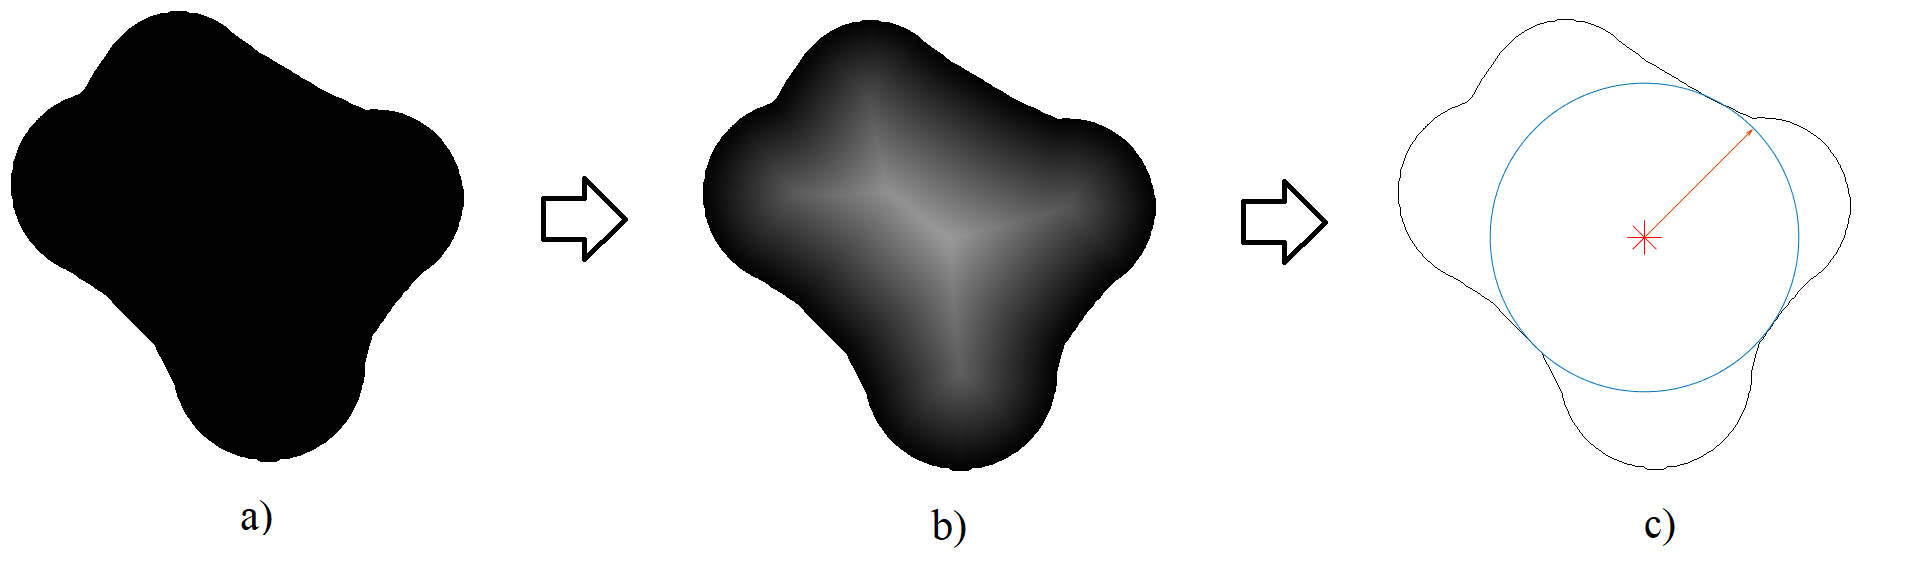
\includegraphics[scale=.42]{figuras/fig3_1.png}
	\caption{Flujo de trabajo para obtener el mayor c�rculo circunscrito.}
	\label{fig:circunFlujo}
\end{figure}

Al haber obtenido el mayor c�rculo circunscrito, ahora se tiene que trazar un c�rculo que se ajuste a cada una de las esquinas, pero antes de eso, se tiene que suavizar el contorno de la part�cula, para evitar que la informaci�n de la rugosidad afecte con el ajuste de los c�rculos. En el art�culo de Zheng \cite{Zheng2016} usan la regresi�n \textit{LOESS} y \textit{k-folds} para suavizar la part�cula, pero nosotros decidimos usar Fourier El�ptico solo tomando en cuenta los primeros 30 arm�nicos de la serie por la facilidad que resulta quitar la informaci�n de la rugosidad.

\begin{figure}[H]
	\centering 
	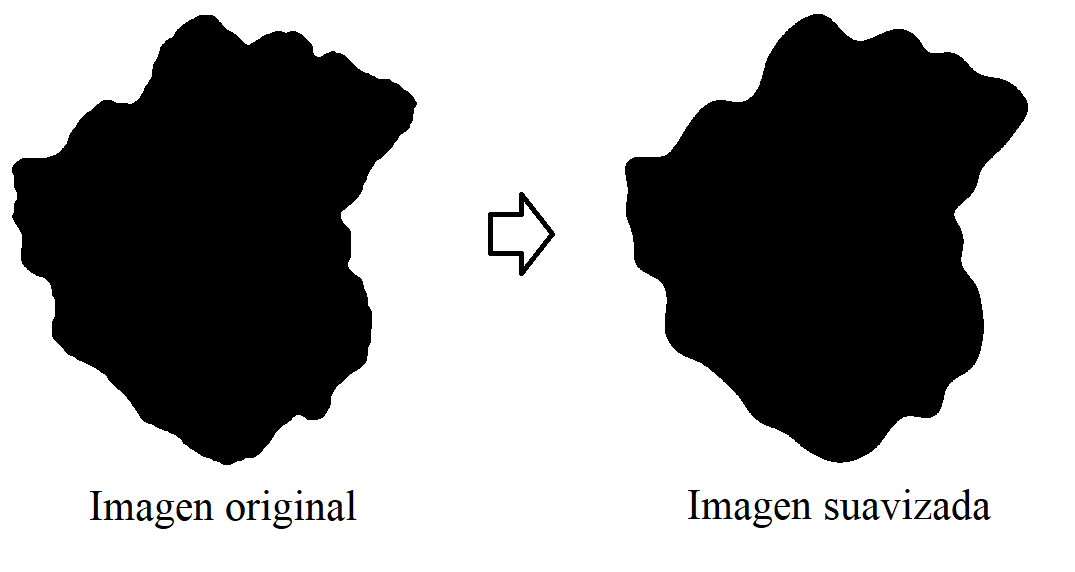
\includegraphics[scale=.42]{figuras/fig3_2.png}
	\caption{Resultado del suavizado de la part�cula utilizando Fourier El�ptico.}
	\label{fig:suavFourier}
\end{figure}

En la figura~\ref{fig:suavFourier}, se observa el suavizado generado por Fourier El�ptico. Para poder identificar las esquinas de la part�cula, se necesita analizar todo el contorno de la part�cula iniciando desde cualquier punto e ir analizando que la sucesi�n de puntos tenga un valor de curvatura positiva, de esta manera se puede discriminar cuando esa curvatura se encuentra por fuera de la part�cula y solo dejando las que est�n por dentro. Para formar los c�rculos, se utiliza una distancia m�xima la cual regula que tan retirados deben de estar los p�xeles del contorno para ser considerados como una sola esquina para despu�s ajustar un c�rculo a todos esos puntos.

\begin{figure}[H]
	\centering 
	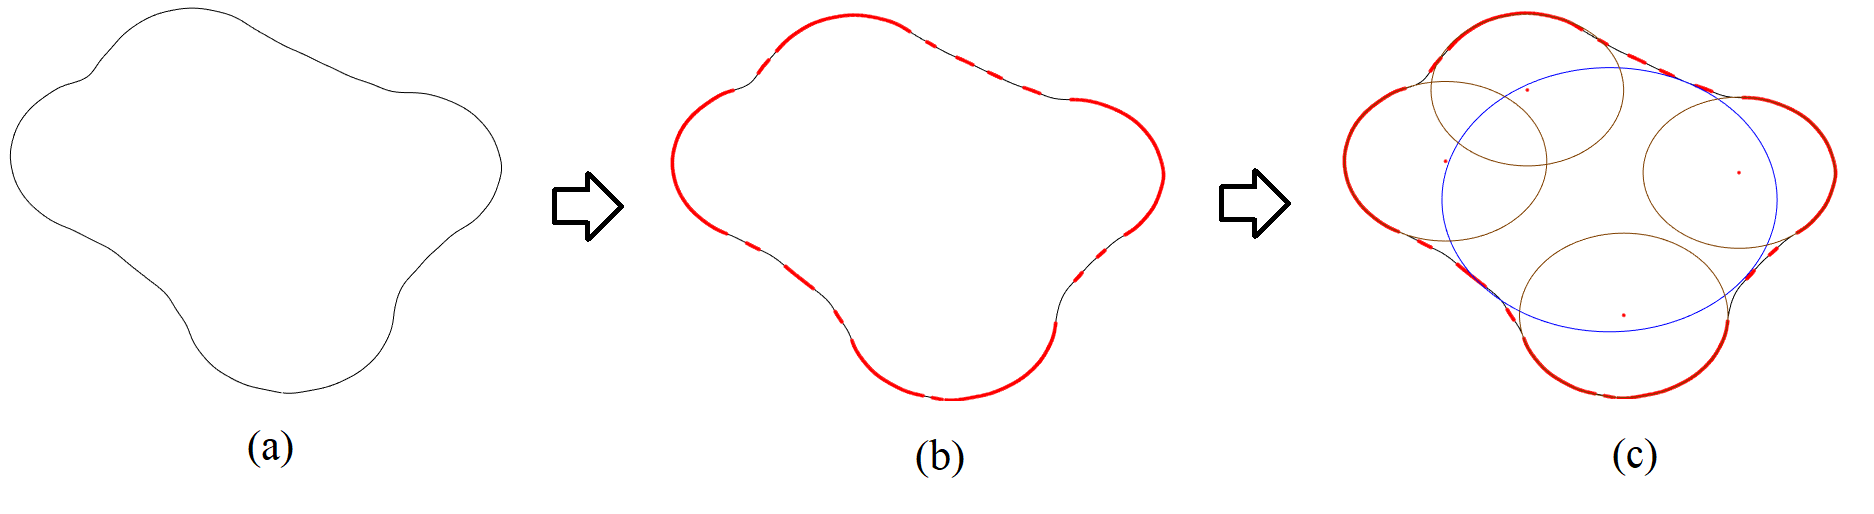
\includegraphics[scale=.42]{figuras/fig3_3.png}
	\caption{Flujo para aproximar las esquinas con c�rculos.}
	\label{fig:flujoCirculos}
\end{figure}

En la Figura~\ref{fig:circunFlujo} se muestra como obtener los c�rculos. (a) tenemos el contorno de la part�cula; (b) remarcamos las  partes del contorno que podr�an ser esquinas utilizando geometr�a computacional; (c) se discriminan regiones seg�ns su curvatura y longitud, as� se seleccionan las esquinas y se ajusta un c�rculo (radio de curvatura) para representarlas.
\begin{equation}
	\label{eqn:roundness}
	\frac{\sum{\frac{r}{R}}}{N} = \text{Grado de redondez}
\end{equation}
Una vez obtenido lo anterior, se pasa a calcular el grado de redondez usando la ecuaci�n ~\ref{eqn:roundness}. El numerador es el promedio de los radios de todos los c�rculos de las esquinas y el denominador corresponde al radio del c�rculo circunscrito m�s grande en la part�cula. El resultado de est� relaci�n es un valor entre 0 y 1, como se describe en el art�culo de Zheng y Hryciw \cite{Zheng2016}.

El mayor inconveniente con este algoritmo es que tres par�metros dependen del tama�o de la part�cula. Un valor mal seleccionado puede producir un error considerable en estimaci�n de la redondez. Los mismo autores sugieren un m�todo para sintonizar estos par�metros, sin embargo, en muchos casos se tiene que realizar una correcci�n manual. Esto reduce el n�mero de im�genes en las que puede funcionar de manera no supervisada.
 
\section{Redes neuronales}

Una red neuronal artificial es un tipo de algoritmo de \textit{Machine Learning} el cual trata de simular el comportamiento del cerebro, al cual le llega una entrada, por medio de neuronas que se activan o no, se obtiene un resultado.

\begin{figure}[H]
	\centering 
	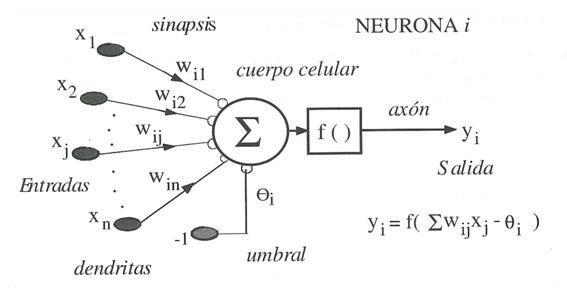
\includegraphics[scale=.8]{figuras/redNeuronal.jpg}
	\caption{Estructura de una neurona artificial an�logo a una biol�gica.}
	\label{fig:estructuraNeurona}
\end{figure}

La neurona es la unidad b�sica, posee dos tareas las cuales son combinar entrada y producir la se�al de activaci�n, siendo un nodo en un grafo dirigido (Red neuronal artificial). La conexi�n entre 2 neuronas es conocida como la sinapsis y su fuerza esta determinada por el est�mulo externo. 

\begin{figure}[H]
	\centering 
	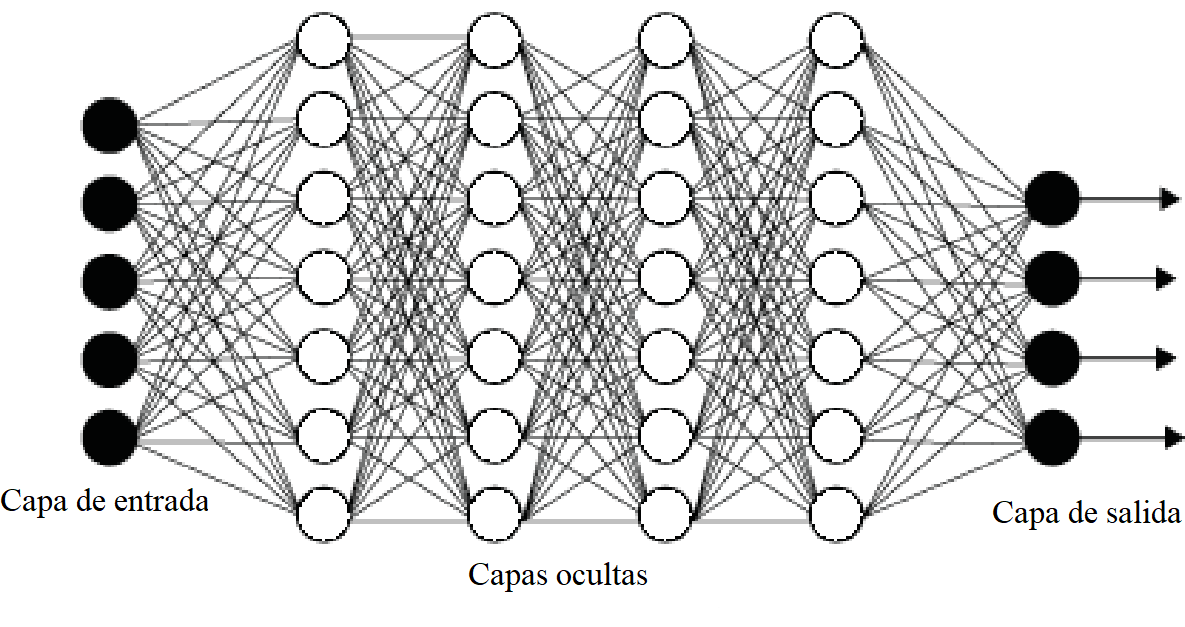
\includegraphics[scale=.5]{figuras/ANN.png}
	\caption{Arquitectura de una red neuronal artificial.}
	\label{fig:arqRedNeuronal}
\end{figure}

Las conexiones o aristas est�n regidas por pesos (\(w_{ij}\)), esos pesos se mezclan con las entradas para producir el "est�mulo", todos los est�mulos de entrada hacia una neurona se combinan para despu�s ingresarlas a la funci�n de activaci�n (\(f()\)) que determinar� la salida hacia la siguiente neurona. En la Figura~\ref{fig:estructuraNeurona} se puede observar los elementos relacionados a una neurona de una red neuronal artificial. 

En la Figura~\ref{fig:arqRedNeuronal} se observa la arquitectura de una red neuronal con su capa de entrada con 4 neuronas, 4 capas ocultas con 7 neuronas cada una, y su capa de salida con 4 neuronas.

\subsection{Funciones de Activaci�n}

Las funciones de activaci�n tienen como objetivo el acotar los valores de salida de una neurona a un cierto rango de valores. La selecci�n de las funciones de activaci�n depender� del problema con el cual se este manejando. Existen funciones lineales y no lineales. Las lineales tienen un uso exclusivo, cuando el problema se trata de regresi�n y solamente en la capa de salida.

\begin{figure}[H]
	\centering 
	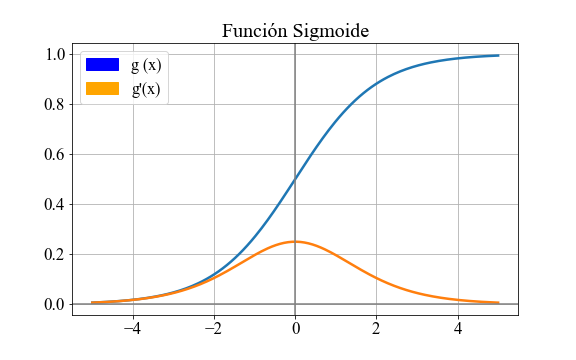
\includegraphics[scale=.6]{figuras/Sigmoid.png}
	\caption{Funci�n de activaci�n Sigmoide.}
	\label{fig:sigmoid}
\end{figure}
\useshortskip
\begin{equation}
	\label{eqn:sigmoid}
	g(x)= \sigma(x)= \frac{1}{1+e^{-x}} \;\;\;\;\;\;\;\; g'(x)= \sigma(x)(1-\sigma(x))
\end{equation} 
La primer funci�n de activaci�n que surgi� fue la Sigmoide, representada en la Figura ~\ref{fig:sigmoid} y expresada por la funci�n \(g(x)\) y su derivada \(g'(x)\) ~\ref{eqn:sigmoid}. Utilizada principalmente para clasificar un conjunto de datos en 2 clases. La utilizaci�n de ella se ha visto mermada porque presenta dos grandes problemas cuando se utiliza como funci�n de activaci�n en las capas ocultas:

\begin{itemize}
	\item Asimetr�a positiva
	\item Desvanecimiento del gradiente
	\item Utilizaci�n de la funci�n exponencial es costoso.
\end{itemize}

La asimetr�a positiva provoca que el gradiente se vuelva ineficiente en la b�squeda del m�nimo, debido a que s�lo puede tomar direcciones totalmente negativas o totalmente positivas, haciendo como una especie de zigzag hasta encontrar el punto m�nimo. El desvanecimiento del gradiente se puede observar en la Figura ~\ref{fig:sigmoid}, ya que, a medida que los valores de x van incrementando, el valor de la derivada va teniendo a 0, provocando que no haya una retroalimentaci�n a la hora de retropropagar hacia atr�s, terminando en que se la red neuronal deje de aprender ya que sus pesos no se van a ir actualizando.

La funci�n se puede seguir usando en la capa de salida pero solo s� el problema lo requiere. Las funciones posteriores trataron de eliminar estos problemas antes mencionados

\begin{figure}[H]
	\centering 
	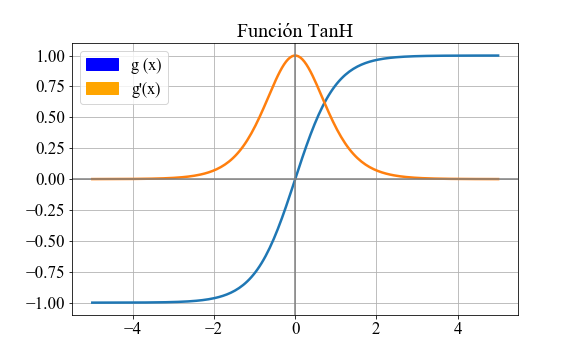
\includegraphics[scale=.6]{figuras/TanH.png}
	\caption{Funci�n de activaci�n Tangente Hiperb�lico.}
	\label{fig:tanh}
\end{figure}
\useshortskip
\begin{equation}
	\label{eqn:tanh}
	g(x)= \tanh{x}=\frac{e^x - e^{-x}}{e^x + e^{-x}} \;\;\;\;\;\;\;\; g'(x)= 1 - \tanh^2{x}=\frac{4}{(e^x+e^{-x})^2}
\end{equation} 
La siguiente funci�n que surgi� fue la Tangente Hiperb�lico (TanH), introducida por LeCun en 1991, representada en la Figura~\ref{fig:tanh}, expresada junto con su derivada en la Ecuaci�n~\ref{eqn:tanh}. Al observar los problemas que presentaba la funci�n Sigmoide, lo que se trataba de encontrar con la funci�n TanH era eliminarlos, sin embargo, solo fue capaz de solucionar el problema de la asimetr�a positiva centrando los datos de -1 a 1, para que el descenso del gradiente fuera m�s eficiente. Sigue presentando los problemas de desvanecimiento del gradiente conforme los valores de \(x\) son m�s grandes, y sigue existiendo el alto costo por usar la funci�n exponencial.

\begin{figure}[H]
	\centering 
	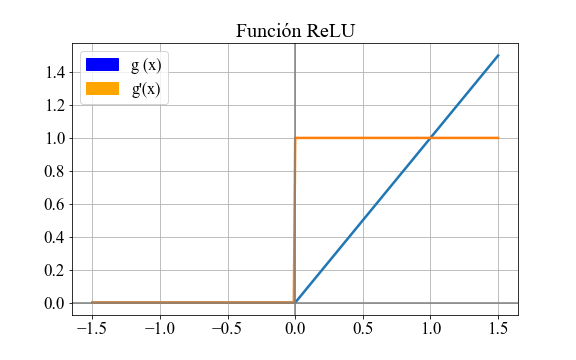
\includegraphics[scale=.6]{figuras/ReLU.png}
	\caption{Funci�n de activaci�n ReLU (Unidad Lineal Rectificada).}
	\label{fig:relu}
\end{figure}
\useshortskip
\begin{equation}
	\label{eqn:relu}
	g(x)= max(0,x) \;\;\;\;\;\;\;\; g'(x)= u(x)
\end{equation} 
La funci�n ReLU o Unidad Lineal Rectificada fue introducida por Vinod Nair en 2010 \cite{nair2010rectified}, representada en la Figura~\ref{fig:relu}, expresada junto a su derivada en la Ecuaci�n~\ref{eqn:relu}, la funci�n \(u(x)\) es el escal�n unitario. Naci� para atacar el problema del desvanecimiento del gradiente, pero sigue conservando, en una menor magnitud, que las otras 2 funciones. Sigue poseyendo el problema de la asimetr�a positiva por no centrar los datos, y se corre el riesgo de que partes de la red neuronal se desconecten si la funci�n empieza a enviar puros ceros, pero tiene la ventaja de que tiene un costo bastante bajo.

Fue muy popular a�os m�s tarde de su nacimiento, pero por los problemas que siguieron existiendo se trat� de buscar una variante la cual controlara o eliminara por completo los problemas, son las siguientes 2 funciones de activaci�n.

\begin{figure}[H]
	\centering 
	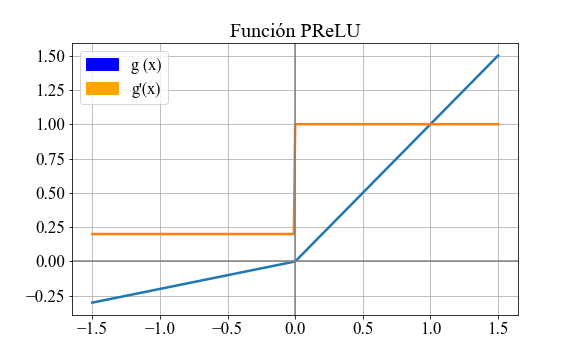
\includegraphics[scale=.6]{figuras/PReLU.png}
	\caption{Funci�n de activaci�n PReLU (Unidad Lineal Rectificada Parametrizada).}
	\label{fig:prelu}
\end{figure}
\useshortskip
\begin{equation}
	\label{eqn:prelu}
	g(x)= max(\alpha x,x) \;\;\;\;\;\;\;\; g'(x) = \alpha + (1-\alpha)u(x)
\end{equation} 
La funci�n PReLU o Unidad Lineal Rectificada Parametrizada fue introducida por Xiangyu Zhang en el a�o 2015 \cite{he2015delving}, representada en la Figura~\ref{fig:prelu}, expresada junto a su derivada en la Ecuaci�n~\ref{eqn:prelu}. El par�metro \(\alpha\) es un coeficiente que va irse adaptando y aprendiendo a lo largo del proceso de aprendizaje de la red neuronal, promoviendo la rapidez del aprendizaje. Ataca principalmente el desvanecimiento del gradiente, ya que la derivada no ser�a cero, y estar�a habiendo retroalimentaci�n en la red, evitando que se desconecten partes de la misma, como a su vez logra reducir la asimetr�a positiva. La funci�n Leaky ReLU es un caso particular de est� funci�n en la cual se igual \(\alpha\) a una constante.

\begin{figure}[H]
	\centering 
	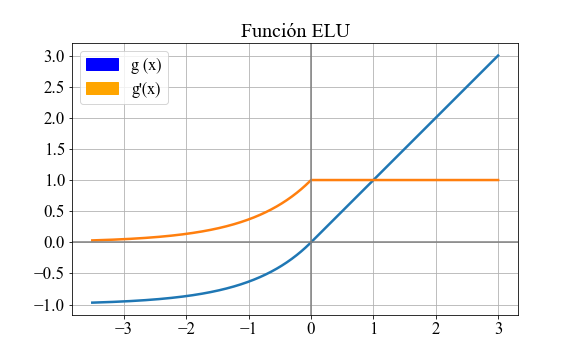
\includegraphics[scale=.6]{figuras/ELU.png}
	\caption{Funci�n de activaci�n ELU (Unidad Lineal Exponencial).}
	\label{fig:elu}
\end{figure}
\useshortskip
\begin{equation}
	\label{eqn:elu}
	g(x)=
	\begin{cases}
	x & x\ge 0\\
	e^x-1 & x<0
	\end{cases}
	\;\;\;\;\;\;\;\;
	g'(x)=
	\begin{cases}
	1 & x\ge 0\\
	e^x & x<0
	\end{cases}
\end{equation} 
Por �ltimo, se tiene la funci�n ELU o Unidad Lineal Exponencial introducido por Djork-Arne Clevert en 2016 \cite{clevert2015fast}. Una gran mejora a comparaci�n de ReLU, ya que no sufre del problema de que se desconecten partes de la red, ataca de mejor manera la asimetr�a positiva, mejora la velocidad de aprendizaje de la red neuronal, a pesar de utilizar la funci�n exponencial y aumentar el tiempo de procesamiento, es un buen trato por obtener una buena funci�n de activaci�n.

Para este trabajo, se tomaron en cuenta las funciones PReLU y ELU por ser las m�s confiables y las que poseen menos problemas, solamente para las capas ocultas. La capa de salida se tom� en cuenta una funci�n lineal de la esfericidad, para verlo como un problema de regresi�n; y para la redondez, se tom� en cuenta la funci�n Softmax para verlo como un problema de clasificaci�n. 

La funci�n Softmax transforma la salida en probabilidades de semejanza que puede tener el sujeto en cuesti�n a cada una de las clases que se tienen, de esta manera, la clase con mayor probabilidad, ser�a la clase definida para ese sujeto.



Los pesos de cada conexi�n entre neuronas se actualiza al final de cada �poca, ese valor esta definido por una funci�n optimizadora que se necesita una velocidad de aprendizaje o \textit{"learning rate"} y una funci�n de error que calcula que tan err�nea fue la salida de la red neuronal con respecto al valor original, si la velocidad de aprendizaje es muy alta, nunca va a encontrar el punto m�nimo debido a que siempre se lo va a pasar y regresar una y otra vez, si el valor es muy peque�o, la funci�n tardar�a demasiado en llegar y quiz�s nunca converja.

Actualmente existen funciones las cuales se les puede asignar un valor de aprendizaje alto pero a su vez asignar un valor de ca�da del aprendizaje, haciendo que en las �poca iniciales sea muy r�pido pero su velocidad vaya bajando gradualmente para ayudar en la convergencia. Tal es el caso de la funci�n RMSprop, que se describen en las siguientes ecuaciones: %~\ref{eqn:rmsprop} est�n sus ecuaciones.
\begin{equation}
	V_{dw}=\beta\cdot V_{dw}+(1-\beta)\cdot dw^2 
\end{equation}
\begin{equation}
	V_{db}=\beta\cdot V_{dw}+(1-\beta)\cdot db^2
\end{equation}
\begin{equation}
	W = W - \alpha\cdot \frac{dw}{\sqrt{V_{dw}}+\epsilon} 
\end{equation}
\begin{equation}
	b = b - \alpha\cdot \frac{db}{\sqrt{V_{db}}+\epsilon}
\end{equation}
La funci�n de error ayuda a la de optimizaci�n a medir el error que hay entre el resultado obtenido y el real, de tal manera que se sepa que tanto se tienen que actualizar los pesos para ir reduciendo el error lo m�s posible.

Una �poca esta definida por la ejecuci�n de cierto flujo de pasos, inicia al ingresar el primer registro de los datos, despu�s actualizar los pesos en base al error, as� hasta acabar con cada uno de los registros, esa es la duraci�n de una �poca.



%\begin{equation}
%\begin{split}
%\label{eqn:rmsprop}
%V_{dw}=\beta\cdot V_{dw}+(1-\beta)\cdot dw^2 \\
%%V_{db}=\beta\cdot V_{dw}+(1-\beta)\cdot db^2 \\
%W = W - \alpha\cdot \frac{dw}{\sqrt{V_{dw}}+\epsilon} \\
%b = b - \alpha\cdot \frac{db}{\sqrt{V_{db}}+\epsilon}
%\end{split}
%\end{equation}         % incluye al archivo Ecuaciones.tex
%
\chapter{Casos de estudió}

\section{Resultados Preliminares}

Resultados de la clasificación de la esfericidad de 1125 partículas.
\begin{figure}[H]
	\centering 
	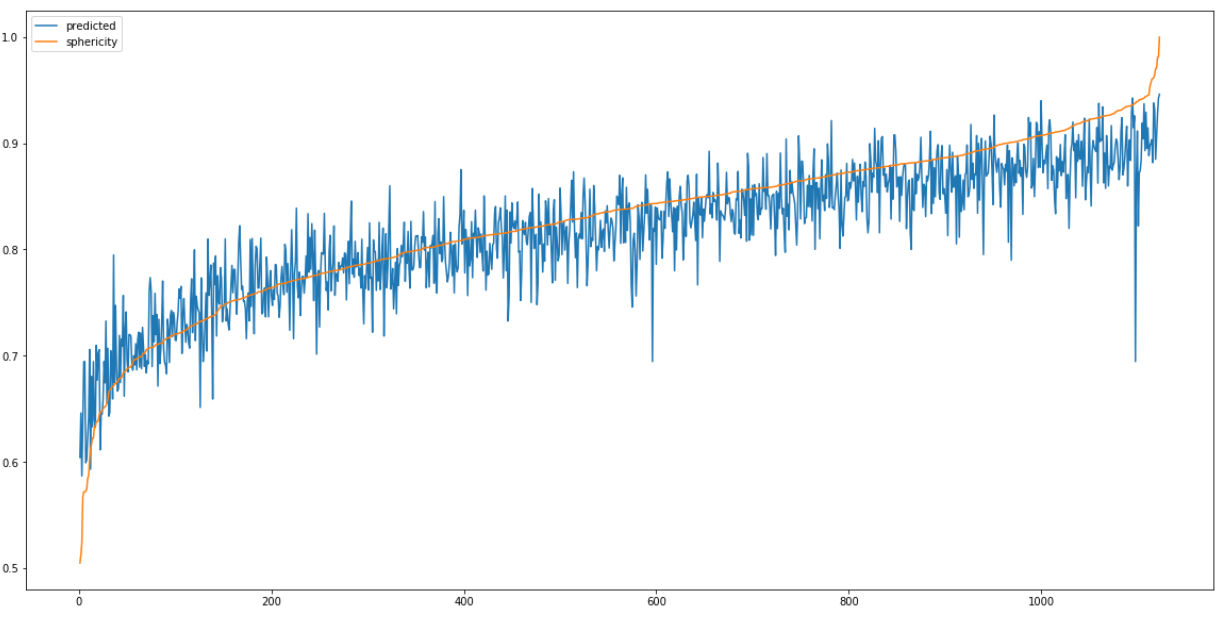
\includegraphics[scale=1]{figuras/resultadosEsfericidad.png}
	\caption{Contraste de la esfericidad obtenidas por la red neuronal contra el valor real.}
\end{figure}

Resultados de la clasificación de la esfericidad de 1125 partículas.
\begin{figure}[H]
	\centering 
	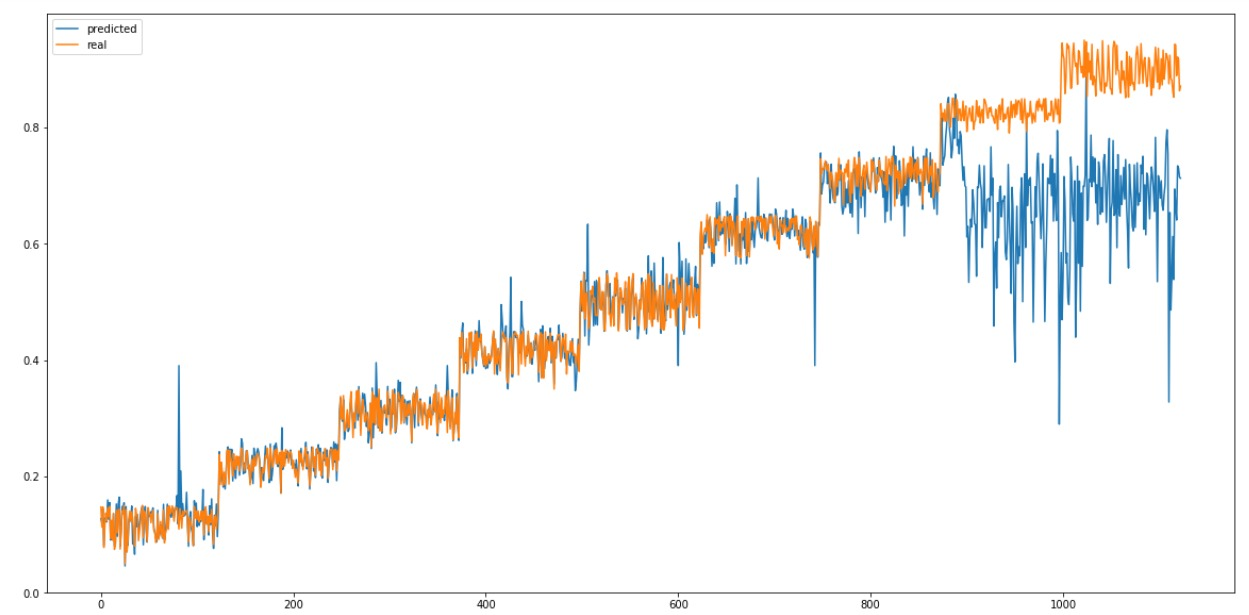
\includegraphics[scale=1]{figuras/resultadosRedondez.jpg}
	\caption{Contraste de la redondez obtenidos por la red neuronal contra el valor real.}
\end{figure} % incluye al archivo Ecuaciones.tex
%\include{Conclusiones}            % incluye al archivo Conclusiones.tex

% ---------------------INTRODUCCIÓN DE APÉNDICES--------------------
% usar \begin{appendix}..\end{appendix} para sólo un apéndice
% usar \begin{appendices}..\end{appendices} para varios apéndices

%\begin{appendices}
%%\include{apenA}                   % incluye al archivo apendA.tex
%%\include{apenB}                   % incluye al archivo apendB.tex
%\end{appendices}

% ------------------INTRODUCCIÓN DE REFERENCIAS---------------------
%\begin{thebibliography}[99]
%\medskip

\printbibliography[title={Referencias}]
%\bibliography{bibliografia}               % incluye al archivo 
%\end{thebibliography}

% ===================================================================
% FINALIZA EL CONTENIDO DEL DOCUMENTO
% ===================================================================

\end{document}